\documentclass[13pt]{beamer}

\usetheme{CambridgeUS}
\usepackage{algorithm}
\usepackage{algpseudocode}
\usepackage{csquotes}
\usepackage{csvsimple}
\usepackage{fontawesome5}
\usepackage{graphicx}
\usepackage{minted}
\usepackage{multicol}
\usepackage{nth}
\usepackage{pgfplots}

\usepackage[backend=biber,style=ieee]{biblatex}
% \addbibresource{references.bib}

\title{Practical Analysis of Hybrid Sorting Algorithms}
\subtitle{Engineering a Faster Standard Sorting Implementation}
\author{Joshua Arulsamy}
\date{May 18, 2023}

\makeatletter
\defbeamertemplate*{footline}{Dan P theme}
{
  \leavevmode%
  \hbox{%
  \begin{beamercolorbox}[wd=.3\paperwidth,ht=2.25ex,dp=1ex,center]{author in head/foot}%
    \usebeamerfont{author in head/foot}\insertshortauthor\expandafter\beamer@ifempty\expandafter{\beamer@shortinstitute}{}{~~(\insertshortinstitute)}
  \end{beamercolorbox}%
  \begin{beamercolorbox}[wd=.4\paperwidth,ht=2.25ex,dp=1ex,center]{title in head/foot}%
    \usebeamerfont{title in head/foot}\insertshorttitle
  \end{beamercolorbox}%
  \begin{beamercolorbox}[wd=.3\paperwidth,ht=2.25ex,dp=1ex,right]{date in head/foot}%
    \usebeamerfont{date in head/foot}\insertshortdate{}\hspace*{2em}
\insertframenumber{} / \inserttotalframenumber\hspace*{2ex}
  \end{beamercolorbox}}%
  \vskip0pt%
}
\makeatother

\begin{document}

% Remove logo
\logo{}
\nocite{*}

\begin{frame}
	\titlepage
\end{frame}

\section{}
\subsection{}
\begin{frame}{Outline}
	\tableofcontents[hideallsubsections]
\end{frame}

\section{Introduction}
\subsection{About Me}
\begin{frame}{About Me}
	\begin{columns}
		\begin{column}{0.5\textwidth}
			\centering
			\makebox[0.7\textwidth]{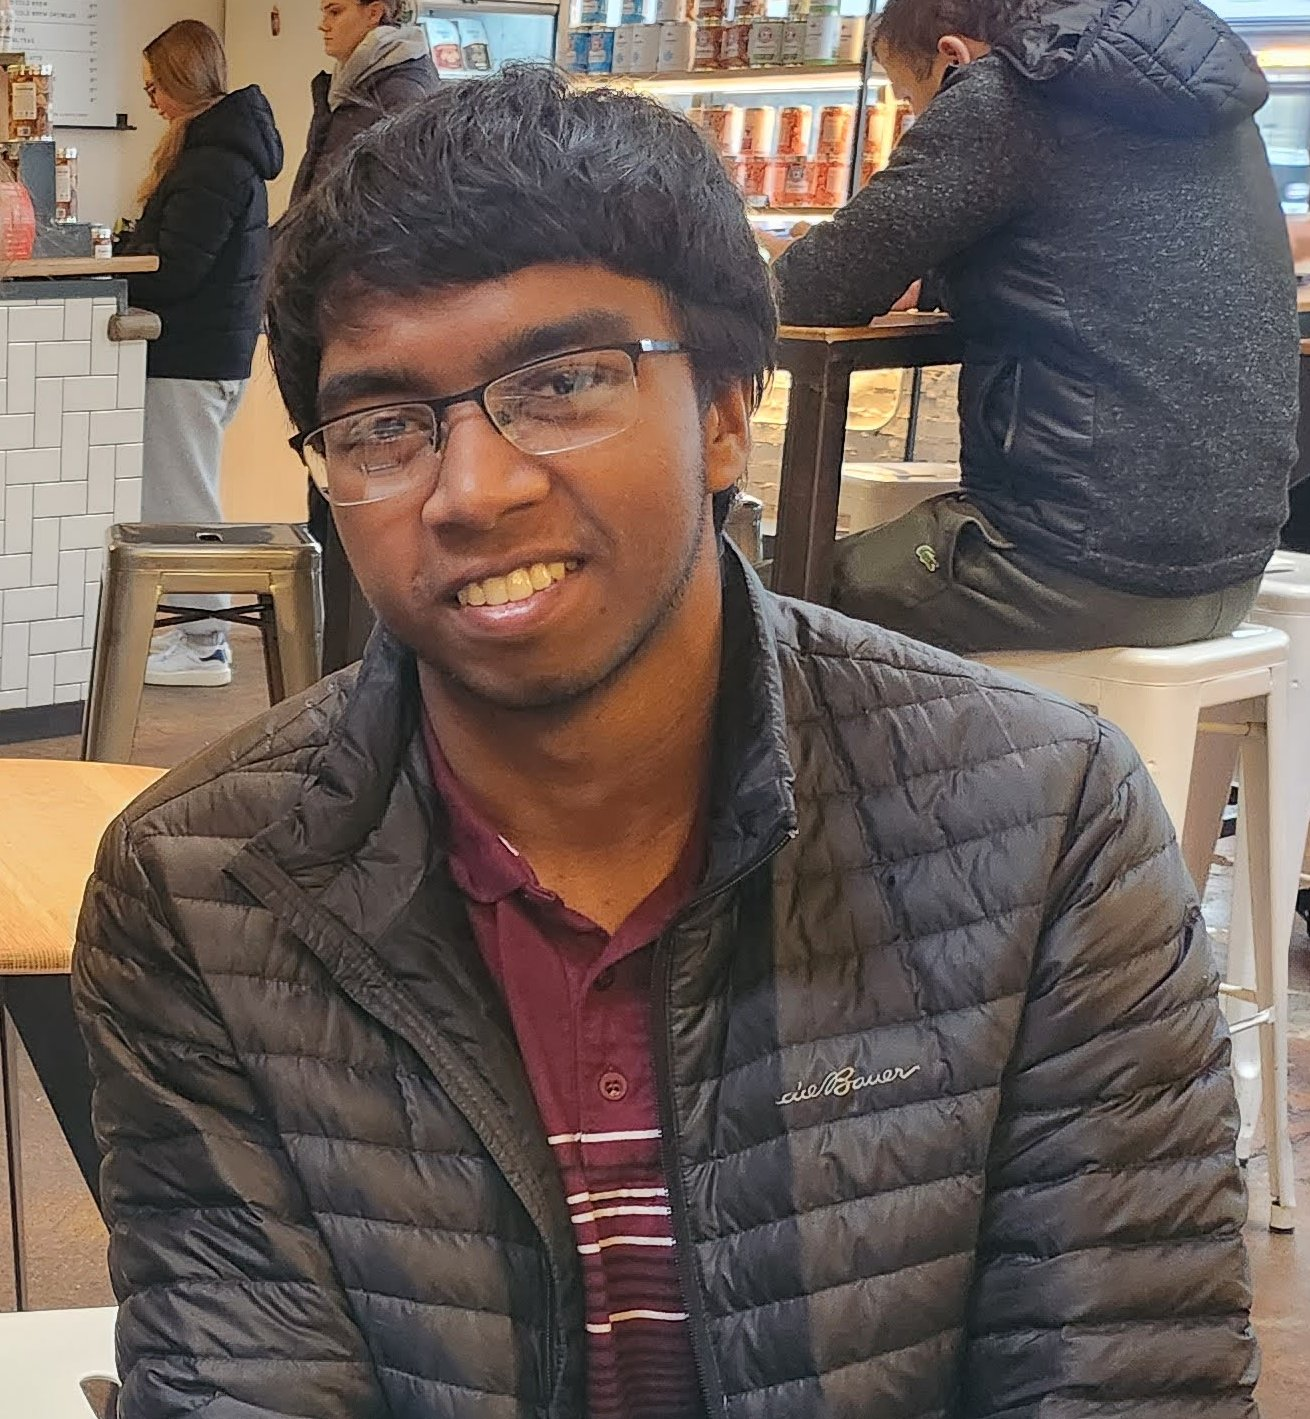
\includegraphics[width=0.7\textwidth,keepaspectratio=true]{./me.jpg}}
		\end{column}

		\begin{column}{0.5\textwidth}
			\begin{itemize}
				\item Graduated Spring 2023 with Bachelors in Computer Science from
				      UW.
				\item Conducted undergraduate research in Dr. Lars Kotthoff's MALLET
				      lab.
				\item Performance optimization, embedded systems, Linux
				      development, system administration.
			\end{itemize}
		\end{column}
	\end{columns}
\end{frame}

\section{Motivation}
\subsection{What's the Deal with Sorting?}
\begin{frame}{What's the Deal with Sorting?}
	\pause
	\begin{itemize}[<+->]
		\item Arguably one of the most researched CS problems.
		\item Many common tasks require sorting somewhere as a step.
		\item Pretty much every programming class covers sorting.
		\item Every programmer must implement sort.
		\item We need fast, standard, type-generic sorting functions in C.
	\end{itemize}
\end{frame}

\subsection{The Existing Solution}
\begin{frame}[c]{The Existing Solution}
	\begin{center}
		\begin{minipage}{0.8\textwidth}
			\inputminted{c}{include.c}
		\end{minipage}

		\pause
		\vspace{0.3cm}
		\begin{displayquote}
			``The \texttt{qsort()} function sorts an array with \texttt{nmemb}
			elements of \texttt{size} size. The \texttt{base} argument points to the
			start of the array.

			The contents of the array are sorted in ascending order according to a
			comparison function pointed to by \texttt{cmp}, which is called with two
			arguments that point to the objects being compared.''
		\end{displayquote}

		\pause
		\textit{Usually} \texttt{qsort()} is implemented using quicksort internally.
	\end{center}
\end{frame}

\section{Vision}
\begin{frame}{Engineering a Faster Version of \texttt{qsort()}}
	\pause
	\begin{enumerate}
		\item Find some fast implementation of quicksort.
		\item Combine it with insertion sort or some other secondary
		      algorithms.
		\item Determine a suitable threshold value to switch to insertion sort
		      internally through copious amounts of testing.
		\item Propose this new implementation to the glibc community.
	\end{enumerate}

	\pause
	\vspace{0.3cm}
	By using a simple algorithm for small arrays, we can avoid some of the
	overhead of more complicated algorithms.
\end{frame}
\begin{frame}{Engineering a Faster Version of \texttt{qsort()}}
	\begin{enumerate}
		\item Find some fast implementation of quicksort.
		\item Combine it with insertion sort or some other secondary
		      algorithms.
		\item \color{red}Determine a suitable threshold value to switch to insertion sort
		      internally through copious amounts of testing.\normalcolor
		\item Propose this new implementation to the glibc community.
	\end{enumerate}

	\vspace{0.3cm}
	By using a simple algorithm for small arrays, we can avoid some of the
	overhead of more complicated algorithms.
\end{frame}


\section{Analyzing Existing Implementations}
\subsection{Quicksort}
\begin{frame}{Why is Quicksort So Popular?}
	\pause
	\begin{itemize}[<+->]
		\item Runs in-place, requires only a constant amount of extra memory.
		\item Fundamentally easy to code and analyze.
		\item Can optimize for corner cases relatively easily.
		\item Fast on average.
		\item Little work on (nearly) sorted data.
		\item Cache friendly.
		\item Maintains a good balance between comparisons and swaps.
	\end{itemize}
\end{frame}

\begin{frame}{Challenges}
	\pause
	\begin{itemize}[<+->]
		\item Worst case $O(n^{2})$ runtime.
		\item Quicksort's performance is primarily dictated by good
		      pivot selection.
		\item Poor pivot selection can adversely affect performance.
		\item Somewhat limited in performance compared to other algorithms
		      which use more memory.
	\end{itemize}
\end{frame}

\subsection{Glibc}
\begin{frame}{When \texttt{qsort()} Isn't Quicksort}
	\begin{itemize}[<+->]
		\item Although the name implies it, \texttt{qsort()} doesn't
		      \textit{have} to use Quicksort internally.
		\item In fact, the C standard imposes no restriction on what
		      algorithms are used internally at all.
		\item Many standard libraries, such as glibc, don't use quicksort
		      all the time anymore.
		\item So, what does glibc use?
	\end{itemize}
\end{frame}

\begin{frame}{Wait, \texttt{qsort()} is Mergesort?}
	\pause
	\begin{itemize}[<+->]
		\item The current \texttt{qsort()} implementation in glibc is recursive
		      mergesort, which automatically falls back to quicksort if memory is
		      limited.
		\item We can leverage memory availability for better performance.
		\item No real downside, we can still operate in memory constrained environments.
	\end{itemize}
\end{frame}

\subsection{Mergesort}
\begin{frame}{Why Use Mergesort Over Quicksort?}
	\pause
	\begin{itemize}[<+->]
		\item Generally easy to implement and reason about.
		\item Worst case $O(n\log{n})$
		\item Uses approximately 30\% less comparisons than quicksort.
		\item Parallelize well.
		\item Stable.
	\end{itemize}
\end{frame}

\section{Performance Optimization}
\subsection{Simple Hybridization}
\begin{frame}{How Can We Make Mergesort Faster?}
	\begin{enumerate}
		\item\pause Reduce recursive overhead and/or number of comparisons
		\begin{itemize}
			\item Apply the same hybridization techniques as with quicksort.
			\item Add an extra tertiary sorting algorithm for even better performance.
		\end{itemize}
		\item\pause Make individual comparisons and swaps faster
		\begin{itemize}[]
			\item Do some alignment trickery.
		\end{itemize}
	\end{enumerate}
\end{frame}

\begin{frame}{How Does Mergesort Work?}
	\begin{algorithmic}
		\Procedure{Mergesort}{$a$}
		\State $n \gets \textnormal{len}(a)$
		\If {$n \le 2$}

		\State sort2(a[0], a[1])

		\Return

		\EndIf
		\State half \gets $\frac{n}{2}$
		\State $lhs \gets a[\textnormal{half}:]$
		\State $rhs \gets a[:\textnormal{half}]$

		\State Mergesort(lhs)

		\State Mergesort(rhs)

		\State Merge(lhs, rhs)
		\EndProcedure
	\end{algorithmic}
\end{frame}

\begin{frame}{How Does Mergesort Work?}
	\begin{columns}
		\begin{column}{0.5\textwidth}
			\begin{algorithmic}
				\Procedure{Mergesort}{$a$}
				\State $n \gets \textnormal{len}(a)$
				\color{red}
				\If {$n \le 2$}

				\State sort2(a[0], a[1])

				\Return

				\EndIf
				\normalcolor
				\State half \gets $\frac{n}{2}$
				\State $lhs \gets a[\textnormal{half}:]$
				\State $rhs \gets a[:\textnormal{half}]$

				\State Mergesort(lhs)

				\State Mergesort(rhs)

				\State Merge(lhs, rhs)
				\EndProcedure
			\end{algorithmic}
		\end{column}
		\begin{column}{0.5\textwidth}
			\pause
			\begin{itemize}[<+->]
				\item Use a secondary algorithm here to limit recursion depth.
				\item Should offer significant performance benefits.
				\item Picking a secondary algorithm is tricky.
			\end{itemize}
		\end{column}
	\end{columns}
\end{frame}

\begin{frame}{Investigating Insertion Sort}
	\begin{itemize}
		\item\pause Anecdotally the best algorithm for this task.
		\item\pause Generally performs very well for small inputs.
		\item\pause Starting from the left:
		\begin{itemize}
			\item Linear search (going backwards) position of current value in sorted subarray on the left.
			\item Insert there.
		\end{itemize}
		\item\pause Worst case: $C(n) = S(n) = \frac{n(n - 1)}{2} \implies O(n^{2})$
		\item\pause Average case: $C_{a}(n) = S_{a}(n) = \frac{n(n - 1)}{4} \implies O(n^{2})$
		\item\pause $C_{a}(32) = S_{a}(32) = 248$
		\item\pause Usually outperforms mergesort for small inputs due to the lack
		of recursive overhead.
	\end{itemize}
\end{frame}

\begin{frame}
	\centering
	\makebox[0.7\columnwidth]{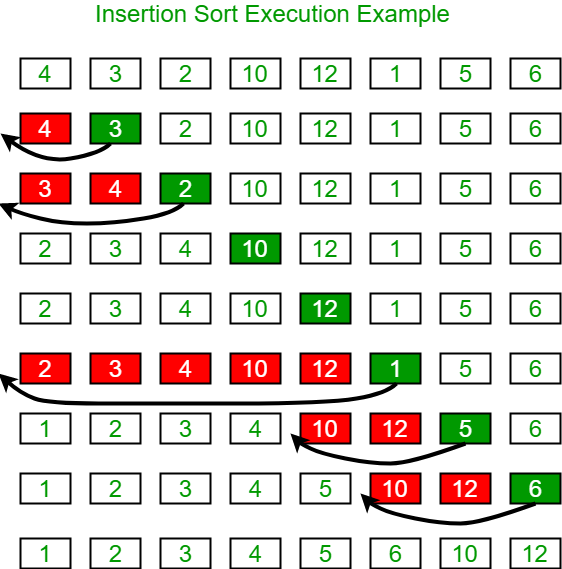
\includegraphics[width=0.7\columnwidth]{./insertionsort.png}}
\end{frame}

\begin{frame}{Why Not Binary Insertion Sort?}
	\pause
	\begin{itemize}[<+->]
		\item Same as normal insertion sort but generally fewer comparisons.
		\item Same number of swaps ($S(n)$)
		\item $C(n) = \sum_{i = 1}^{n - 1}{\lceil \log_{2}{i} \rceil}$
		\item $C(32) = 155$ (compared to 248)
		\item Less work for the same result!
	\end{itemize}
\end{frame}

\begin{frame}{Some Microbenchmarks}
	\begin{itemize}
		\item Test on 1M random \texttt{doubles}, threshold 32.
		\item Insertion sort: 25.33M comparisons.
		\item Binary Insertion Sort: 22.14M comparisons.
		\item Same number of swaps (13.79M)
	\end{itemize}
\end{frame}

\begin{frame}{Oops...}
	\begin{itemize}[<+->]
		\item Insertion Sort: 60.75 ms.
		\item Binary Insertion Sort 68.58 ms.
		\item 13\%... slower?
		\item Increasing threshold only yields worse performance.
	\end{itemize}
\end{frame}

\begin{frame}{Modern Branch Prediction is to Blame}
	\begin{displayquote}
		``Digital circuit that tries to guess which way a branch (e.g., an
		if–then–else structure) will go before this is known definitively.''
	\end{displayquote}

	\begin{itemize}
		\item\pause Linear searches are highly predictable.
		\begin{itemize}
			\item Literally only one fail can occur per search.
			\item Average success rate: $R(n) = \frac{n - 4}{n}$\\
			      R(32) = 87.5\%
			\item Branch prediction works swimmingly.
		\end{itemize}
		\item\pause Binary searches frequently switch which conditional path is taken.
		\begin{itemize}
			\item Each iteration extracts 1 bit of information.
			\item Average success: $R(n) = 50\%$
			\item Branch prediction is ineffective.
		\end{itemize}
	\end{itemize}
\end{frame}

\subsection{Realization}
\begin{frame}{Realization}
	\begin{itemize}[<+->]
		\item Existing research suggesting minimizing comparisons while provide
		      optimal performance.
		\item As we've seen, this isn't necessarily true.
		\item Extracting max info per comparison is the primary goal.
		\item External factors, like branch predictors, can adversely affect
		      performance.
	\end{itemize}
\end{frame}

\begin{frame}{Realization}
	\centering
	\Huge The only way to be sure is to test, test, and test some more!
\end{frame}

\subsection{Testing Secondary Algorithms}
\begin{frame}{Testing Secondary Algorithms}
	\begin{itemize}
		\item A small selection of algorithms were chosen to test with mergesort
		      and quicksort hybridization:
		      \begin{itemize}
			      \item Insertion sort
			      \item Binary insertion sort
			      \item Shell sort
			      \item Sorting Networks
			      \item Bubble Sort
			      \item Heapsort
		      \end{itemize}
		      \item\pause Many of these were immediately discarded for a variety of reasons.
		      \item\pause Various threshold values were evaluated to find the best
		      algorithm configuration.
		      \item\pause Tests were on various types of data and repeated on several
		      platforms.
		      \item\pause Of these algorithms, insertion sort paired with sorting
		      networks generally performed the best.
	\end{itemize}
\end{frame}

\subsection{Sorting Networks}
\begin{frame}{What Are Sorting Networks?}
	\begin{itemize}
		\item Consists of two items, comparators and wires.
		\item Wires run left to right.
		\item When a pair of values encounter a comparator, the comparator swaps the
		      values if the top wire value is greater than or equal to the bottom
		      wire's value.
	\end{itemize}

	\centering
	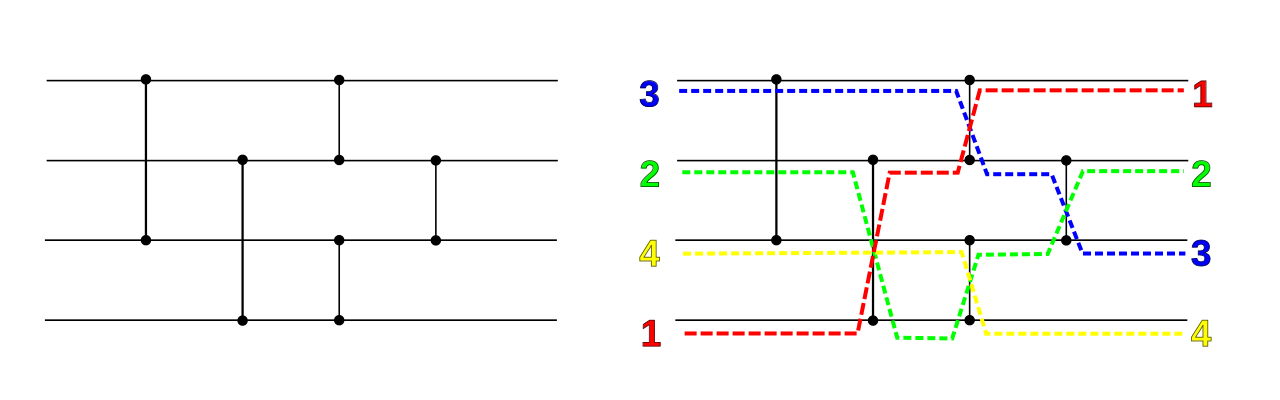
\includegraphics[width=0.8\columnwidth]{simplesortingnetwork.png}
\end{frame}

\begin{frame}{What Makes Sorting Networks So Fast?}
	\pause
	\begin{itemize}[<+->]
		\item Unlike conventional sorting algorithms, sorting networks can only
		      sort a fixed number of items.
		\item Depth and comparison optimal sorting networks have been
		      mathematically proven for small input sizes ($n \le 13$).
		\item Comparison optimal networks save expensive function calls to
		      comparator functions.
		\item Networks are very branch and cache friendly, and even parallelize
		      well.
	\end{itemize}
\end{frame}

\begin{frame}{What Do We Have So Far?}
	\begin{enumerate}
		\item Use recursive mergesort instead of quicksort.
		\item Use sorting networks for very small subarrays.
		\item Use insertion sorting for medium-sized subarrays.
	\end{enumerate}
\end{frame}


\subsection{Alignment Trickery}
\begin{frame}{The Final Step - Alignment Trickery}
	\begin{itemize}[<+->]
		\item Using some \texttt{gcc} macro magic, we can determine the alignment
		      of the input data \textit{at runtime} very cheaply.
		\item Paired with the size of each element we can mimic primitives during
		      the sorting process.
		\item We can avoid \textit{many} system calls!
		\item This has a significant performance impact.
		\item We can fallback to the generic system call solution for any
		      nonprimitive.
	\end{itemize}
\end{frame}

\begin{frame}{Why is This Faster?}
	\begin{displayquote}
		``If it is aligned like an \texttt{int} and sized like an \texttt{int}
		it is an \texttt{int}.''
	\end{displayquote}
	\begin{center}
		\begin{minipage}{0.7\textwidth}
			\inputminted[fontsize=\scriptsize]{c}{alignmenttricks.c}
		\end{minipage}
	\end{center}
\end{frame}

\section{The New Algorithm}
\begin{frame}{The New Algorithm}
	\pause
	\begin{itemize}[<+->]
		\item Highly optimized, cache friendly, recursive merge sort.
		\item Use sorting networks for inputs smaller than $n = 4$.
		\item Use insertion sort for inputs around size 16, depending on the
		      platform.
		\item Use alignment trickery for optimized swapping.
	\end{itemize}
\end{frame}

\subsection{Results}
\begin{frame}{Results - Random Data}
	\begin{multicols}{2}
		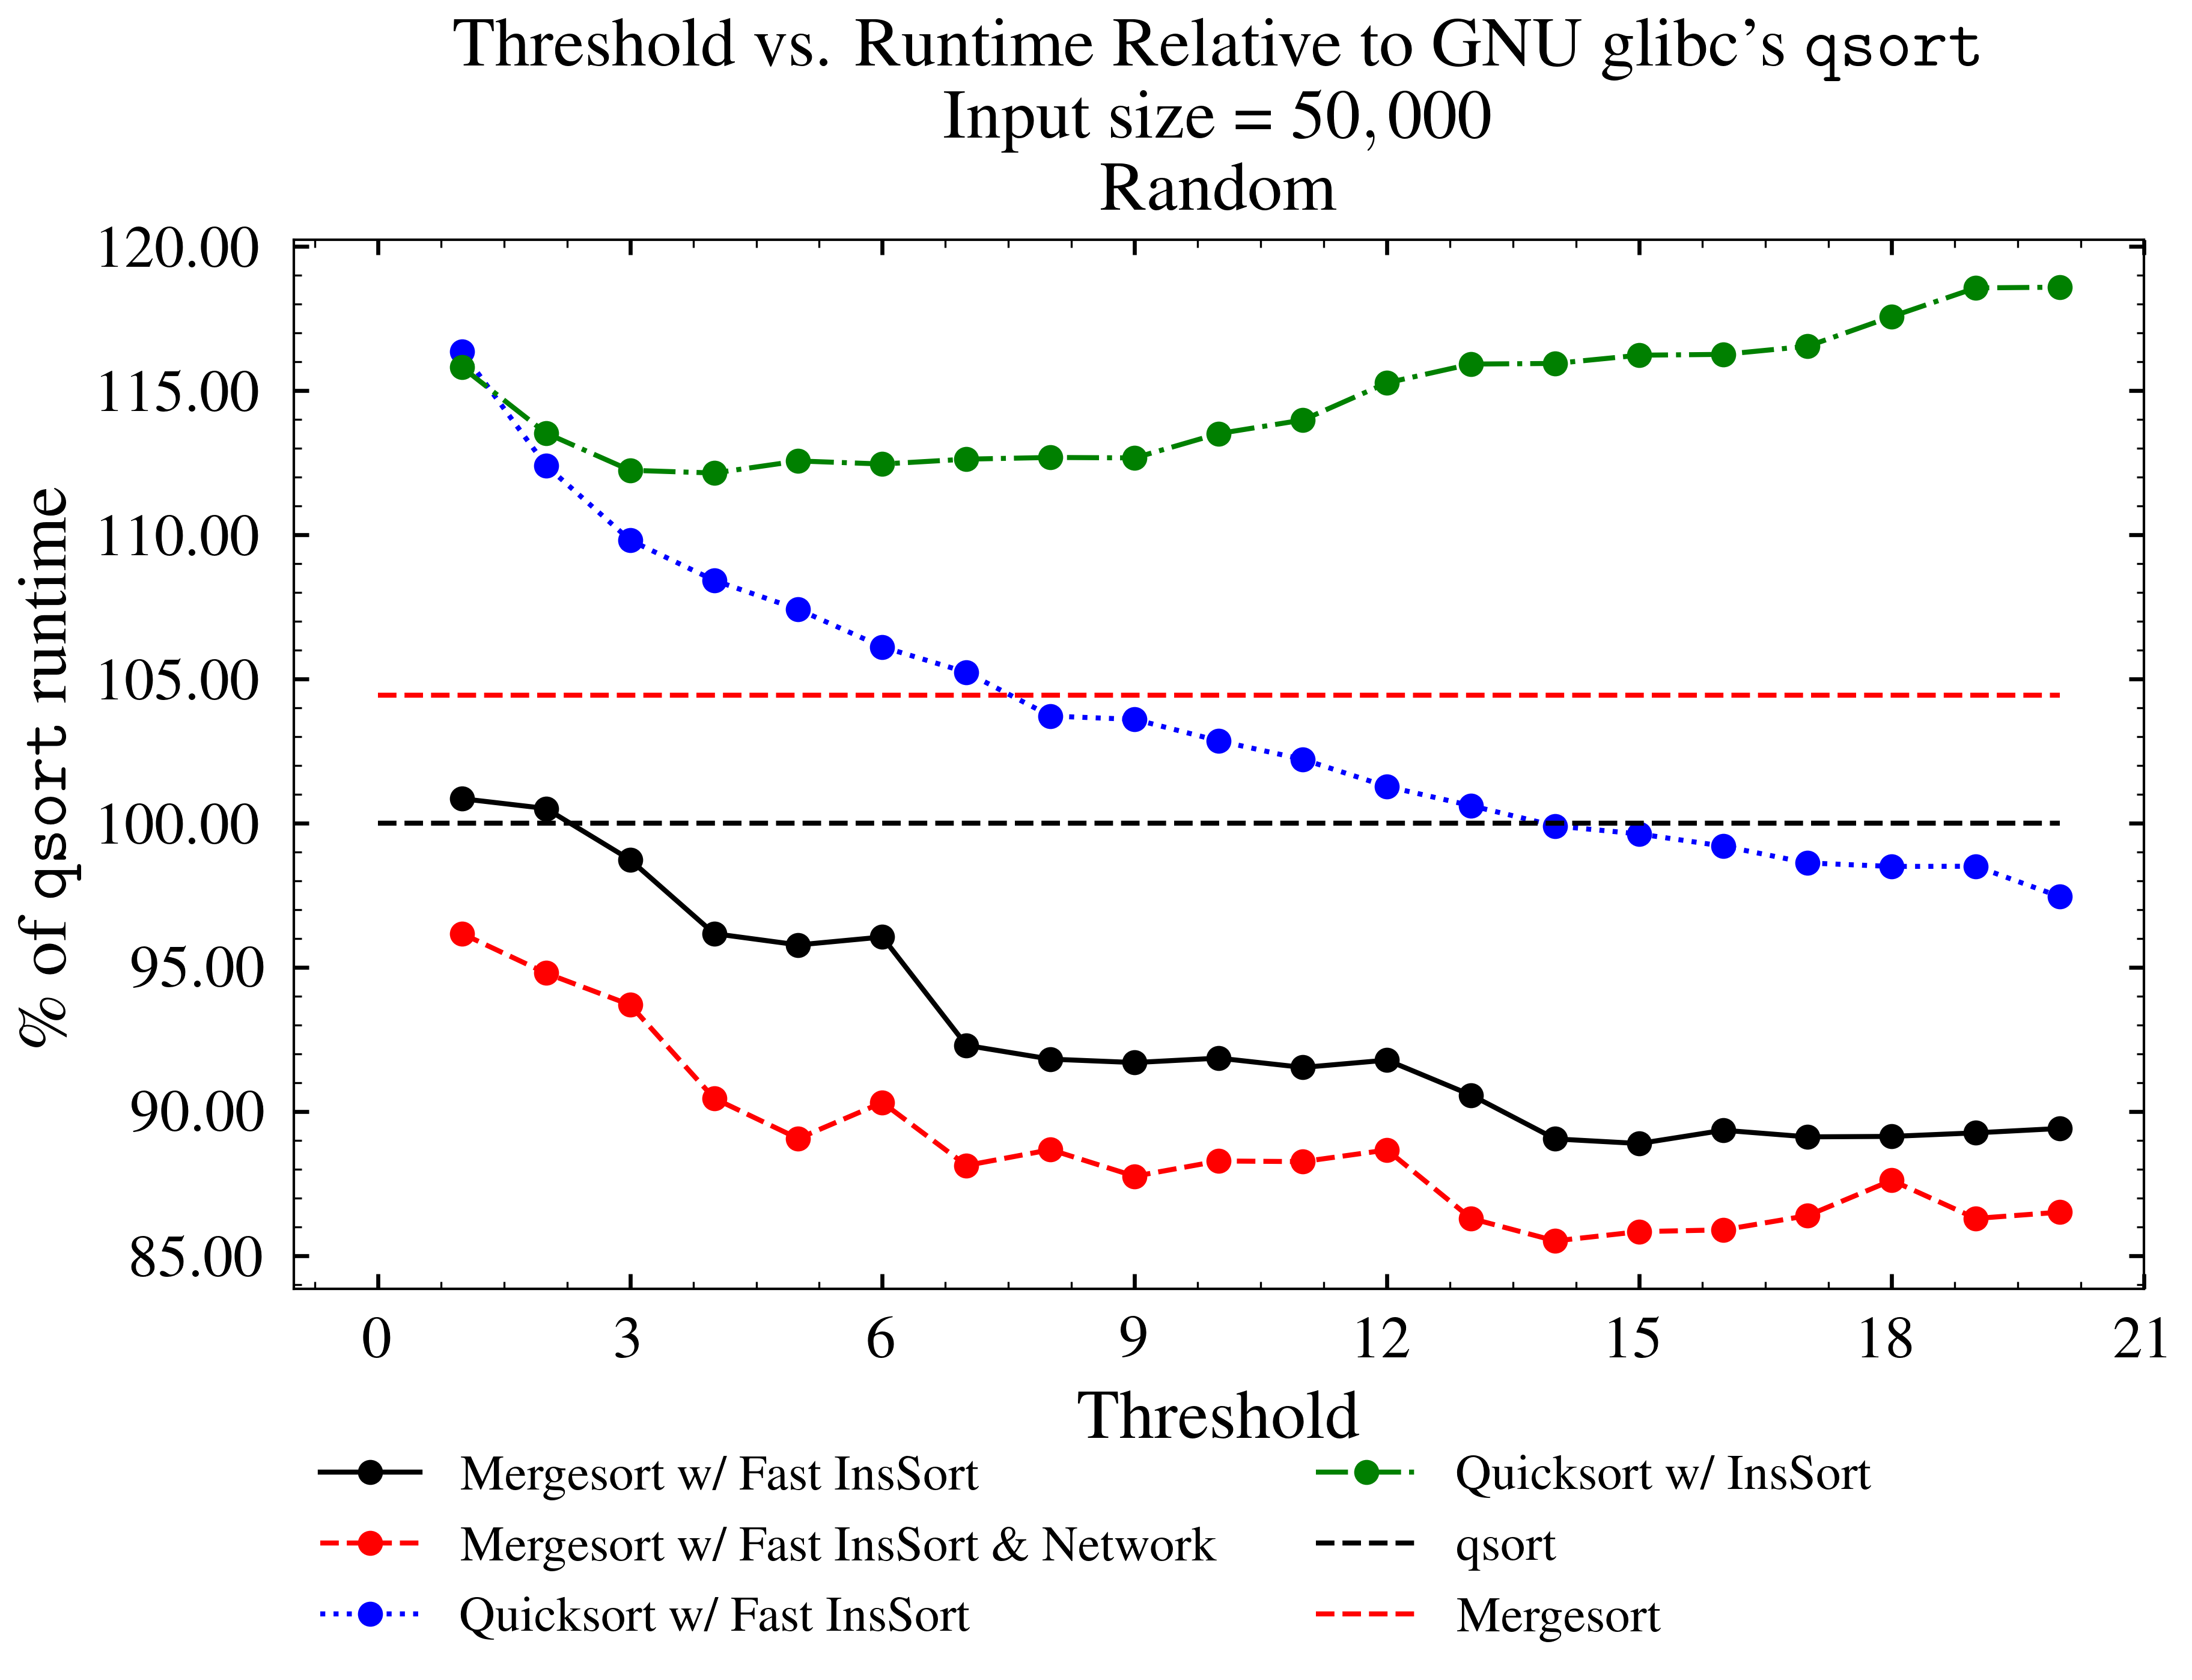
\includegraphics[width=\columnwidth]{../figures/random.png}
		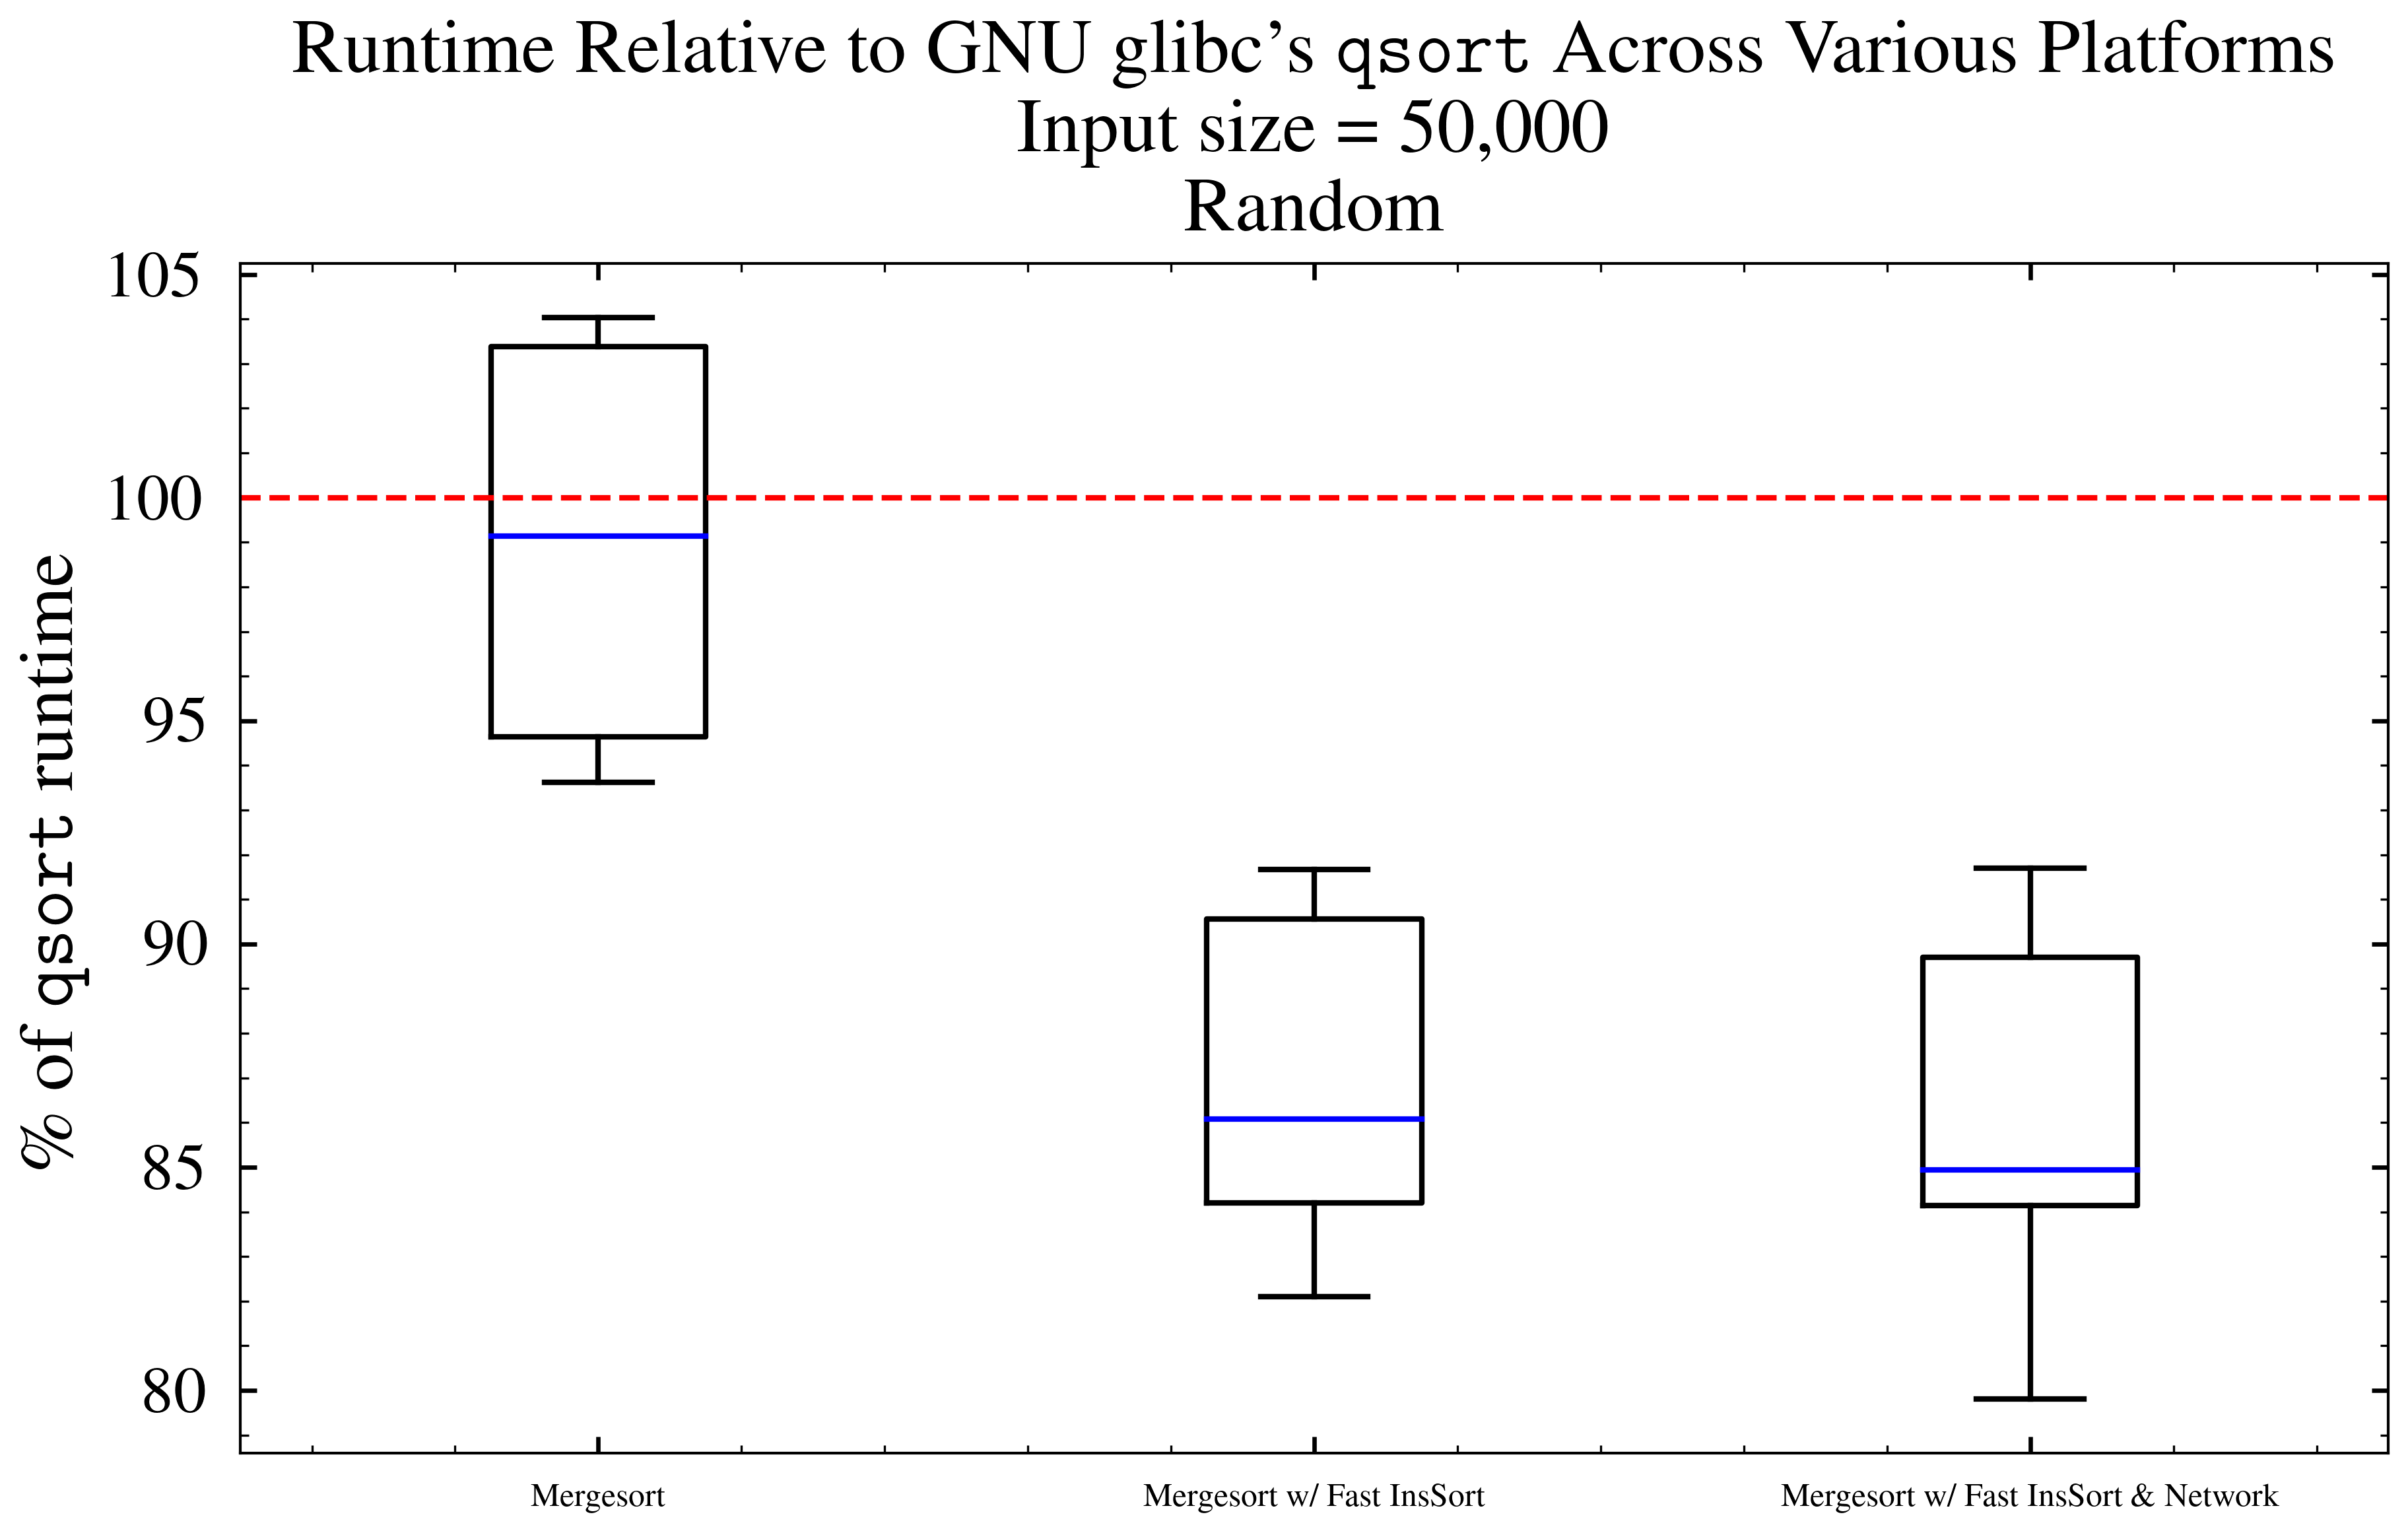
\includegraphics[width=\columnwidth]{../figures/boxplots/4.gen.png}
	\end{multicols}
\end{frame}

\begin{frame}{Results - Ascending Data}
	\begin{multicols}{2}
		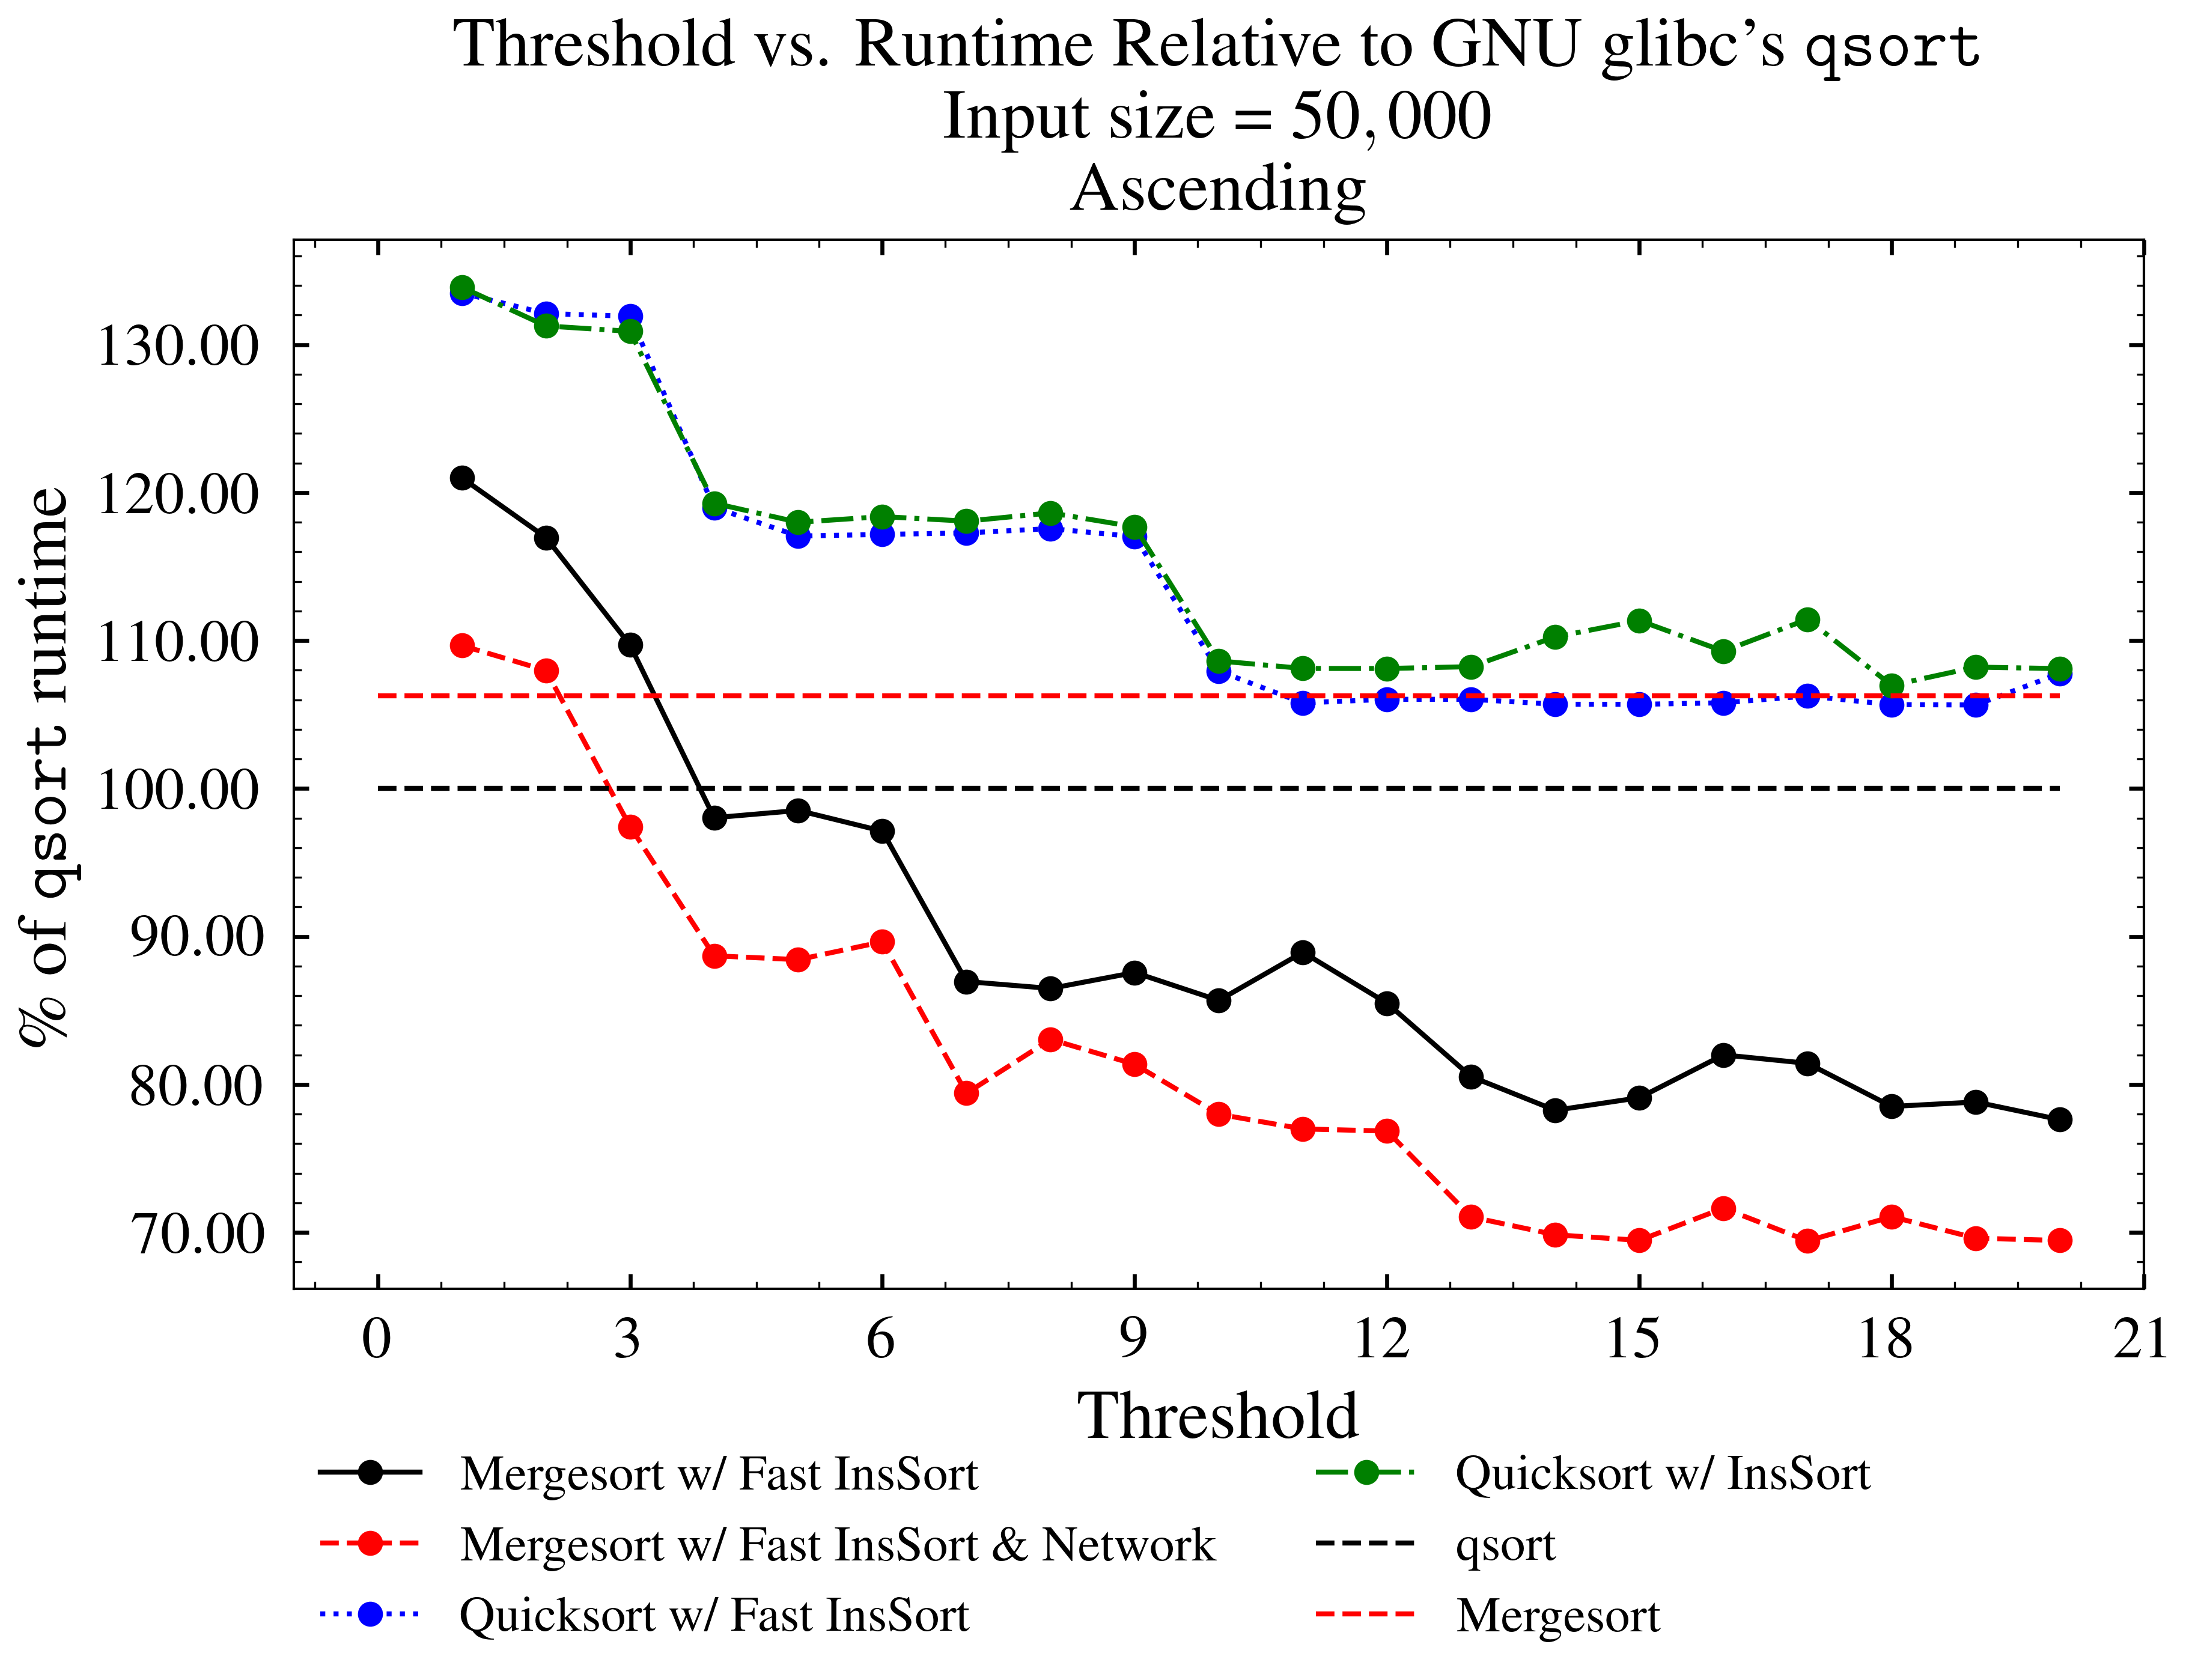
\includegraphics[width=\columnwidth]{../figures/ascending.png}
		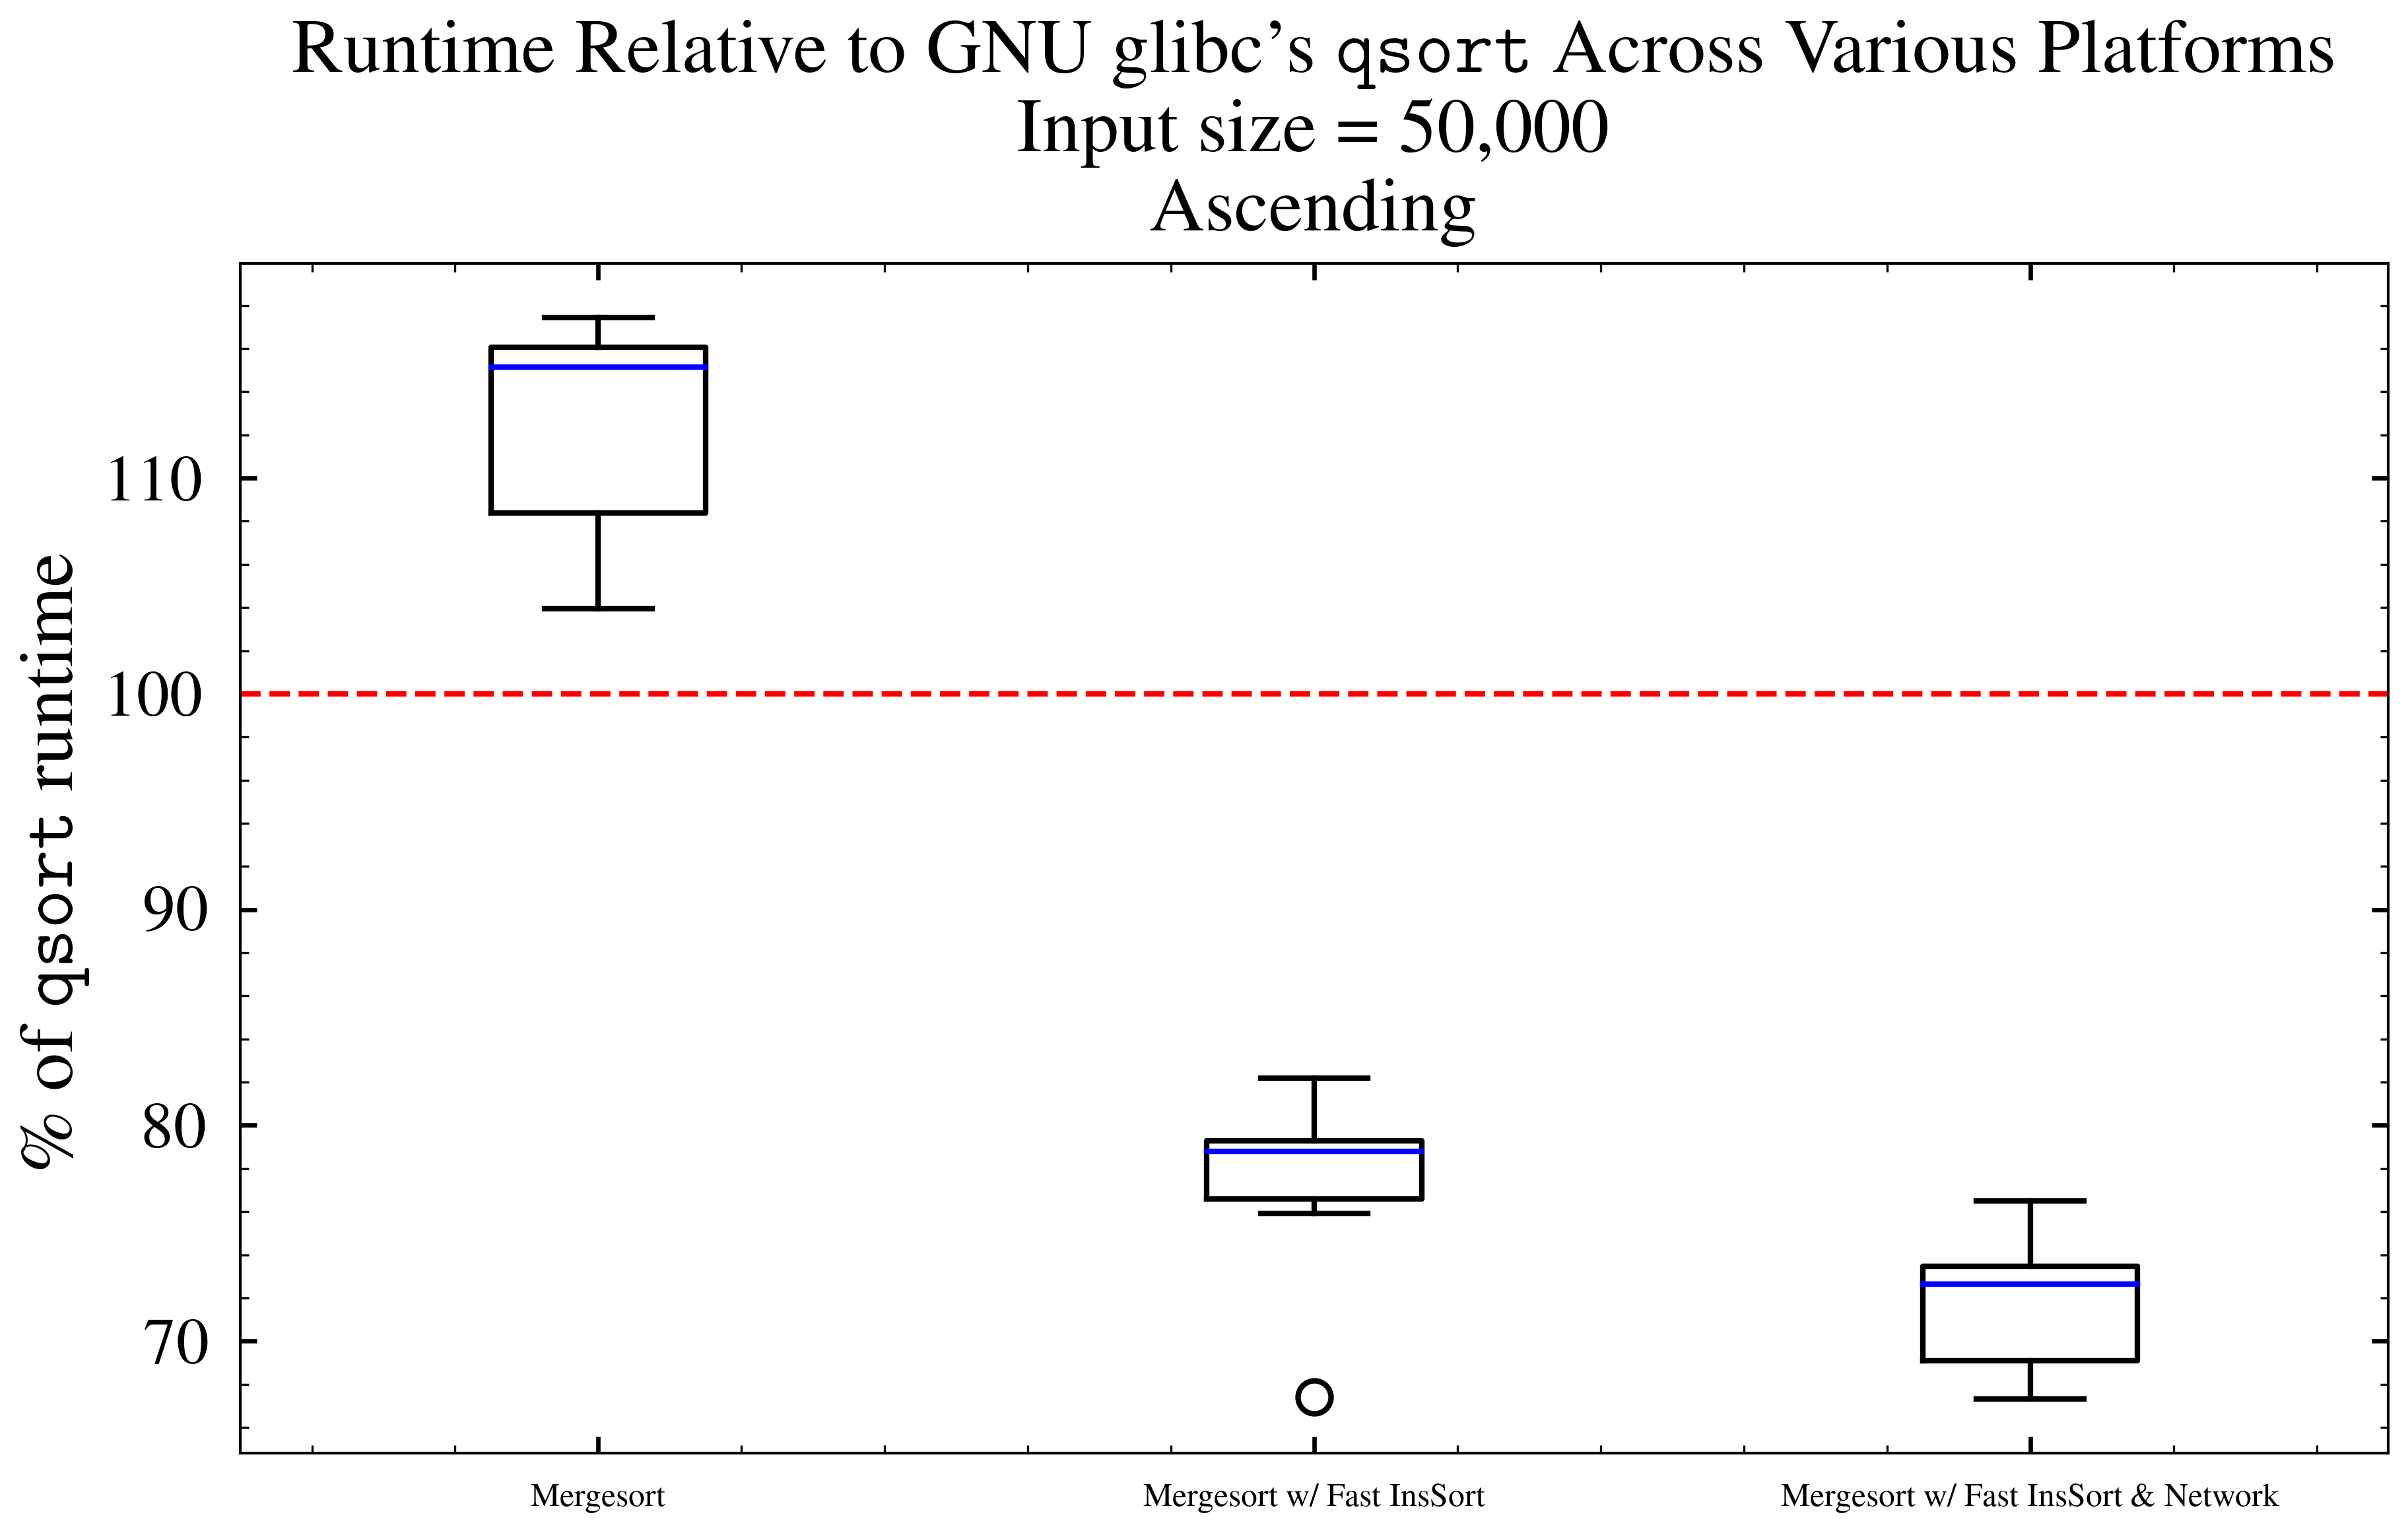
\includegraphics[width=\columnwidth]{../figures/boxplots/2.gen.png}
	\end{multicols}
\end{frame}

\begin{frame}{Results - Descending Data}
	\begin{multicols}{2}
		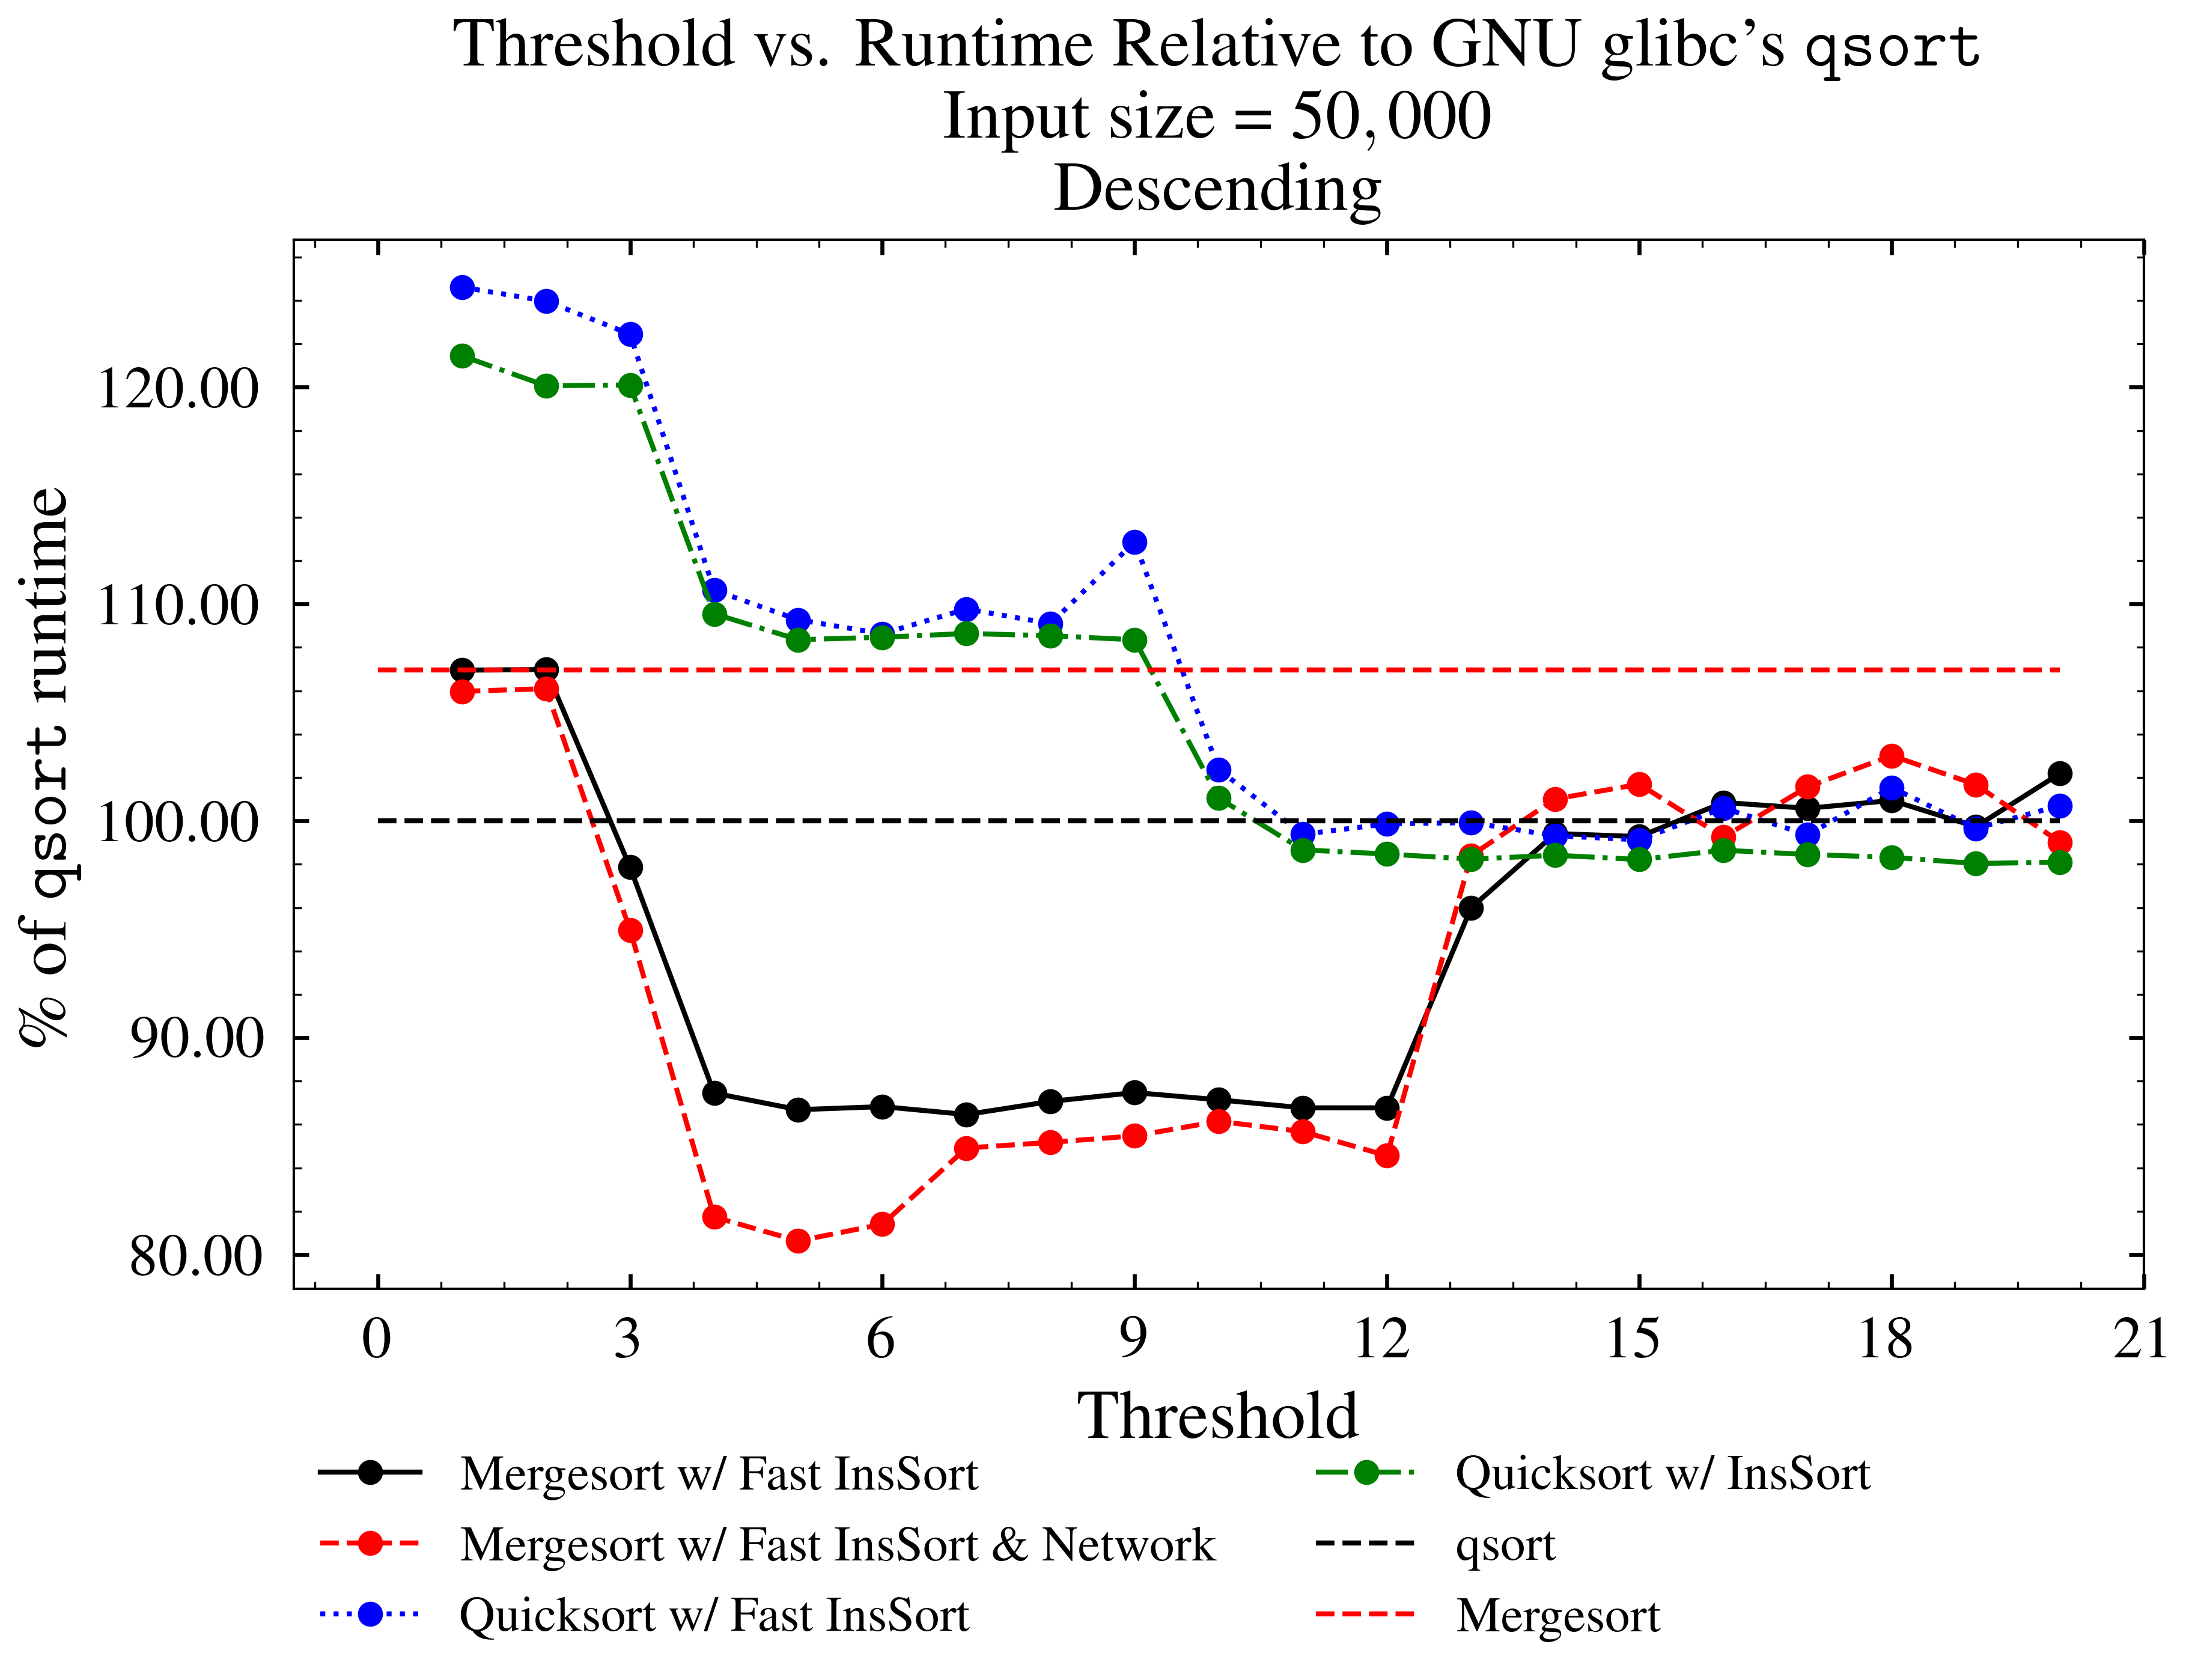
\includegraphics[width=\columnwidth]{../figures/descending.png}
		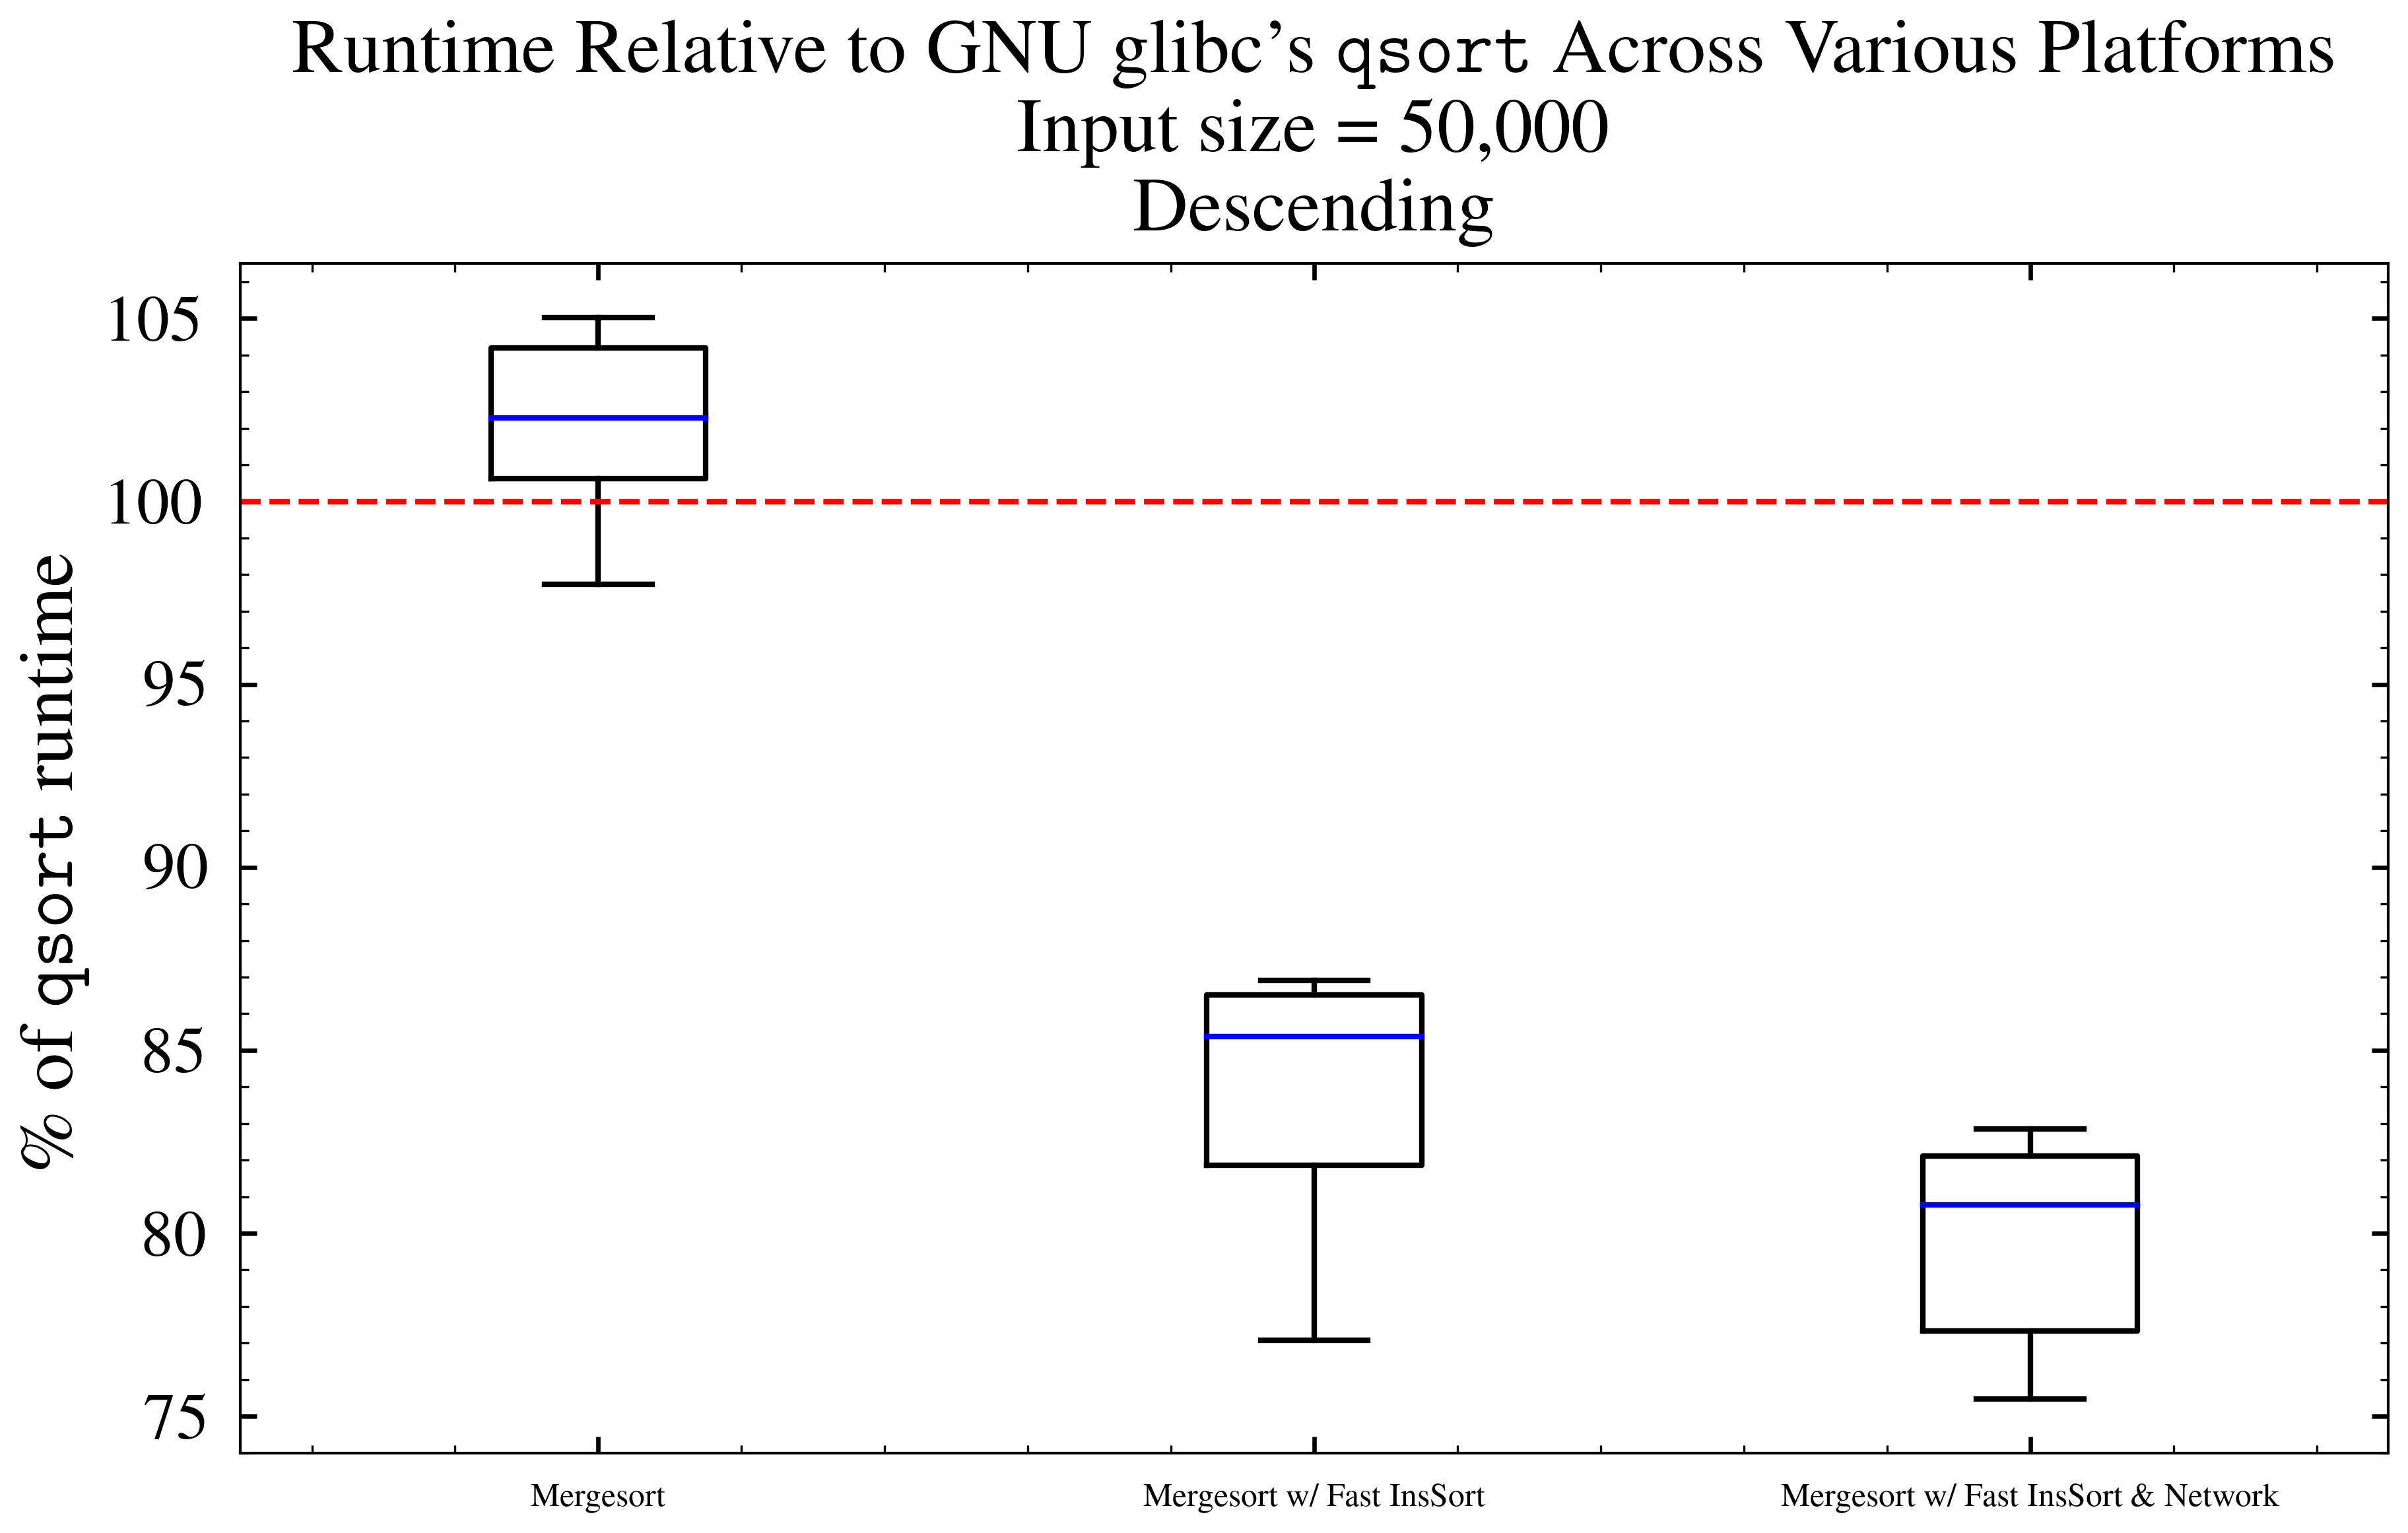
\includegraphics[width=\columnwidth]{../figures/boxplots/3.gen.png}
	\end{multicols}
\end{frame}

\begin{frame}{Results - Repeated Single Num Data}
	\begin{multicols}{2}
		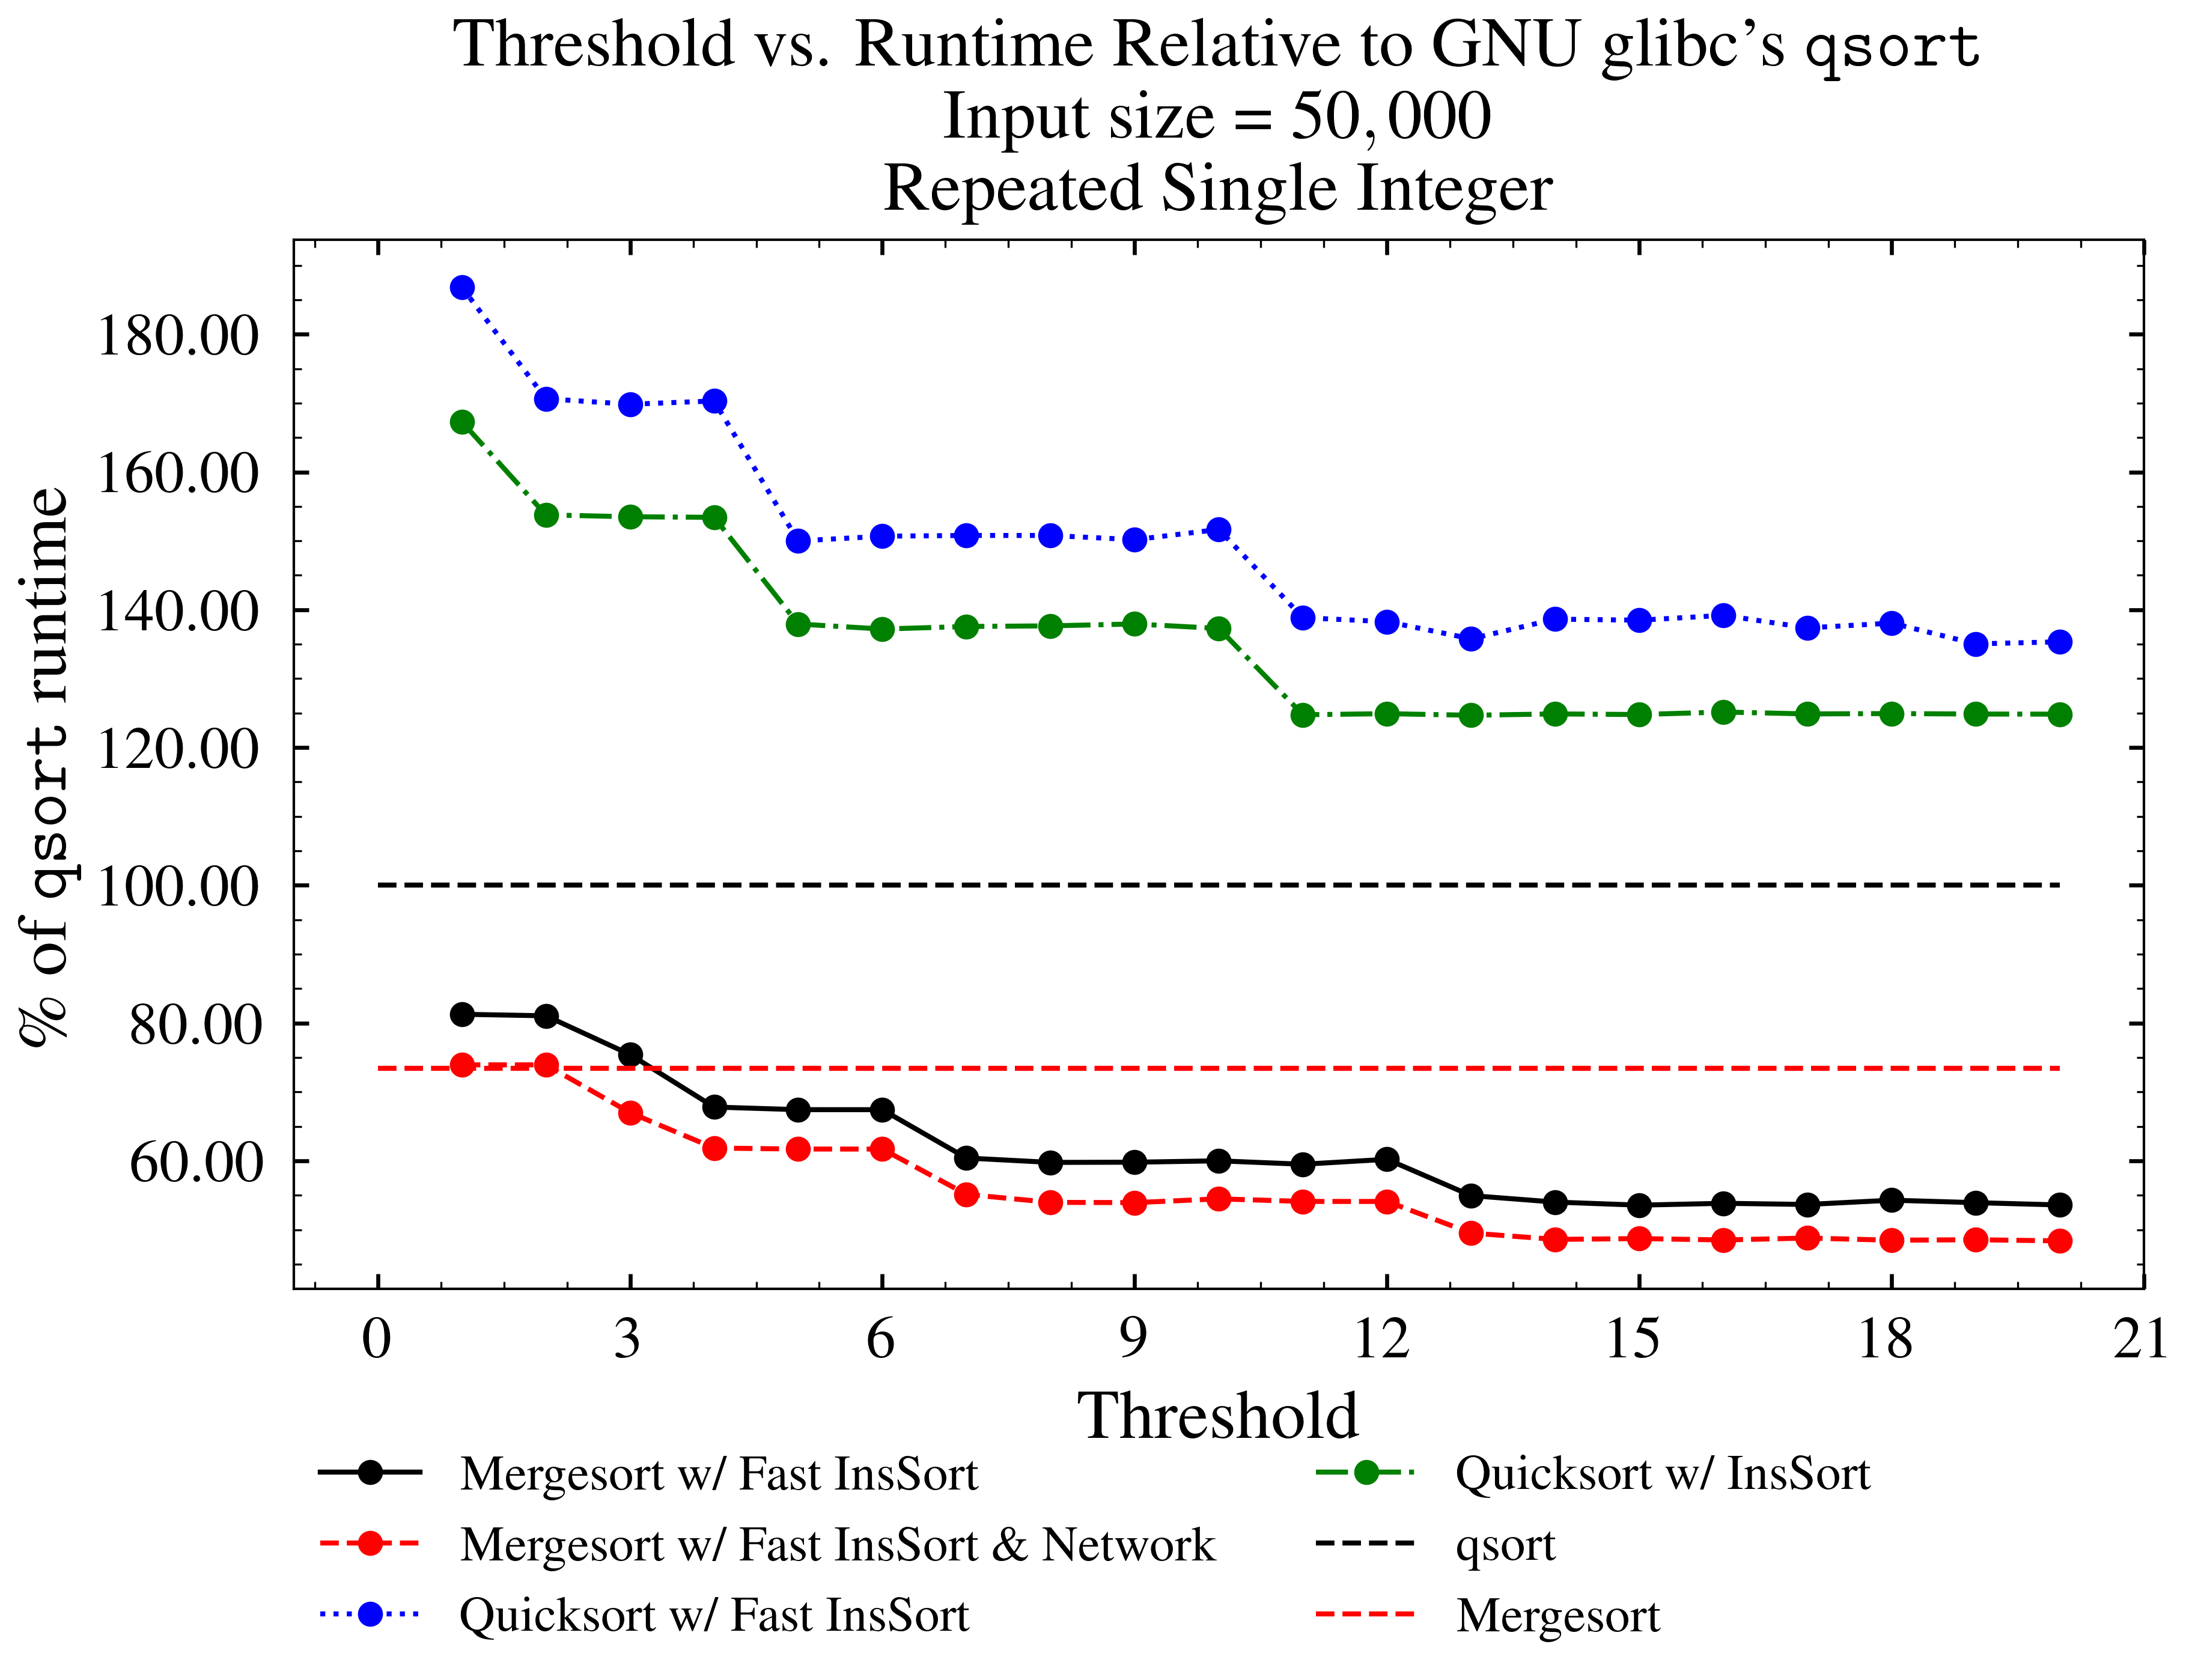
\includegraphics[width=\columnwidth]{../figures/single_num.png}
		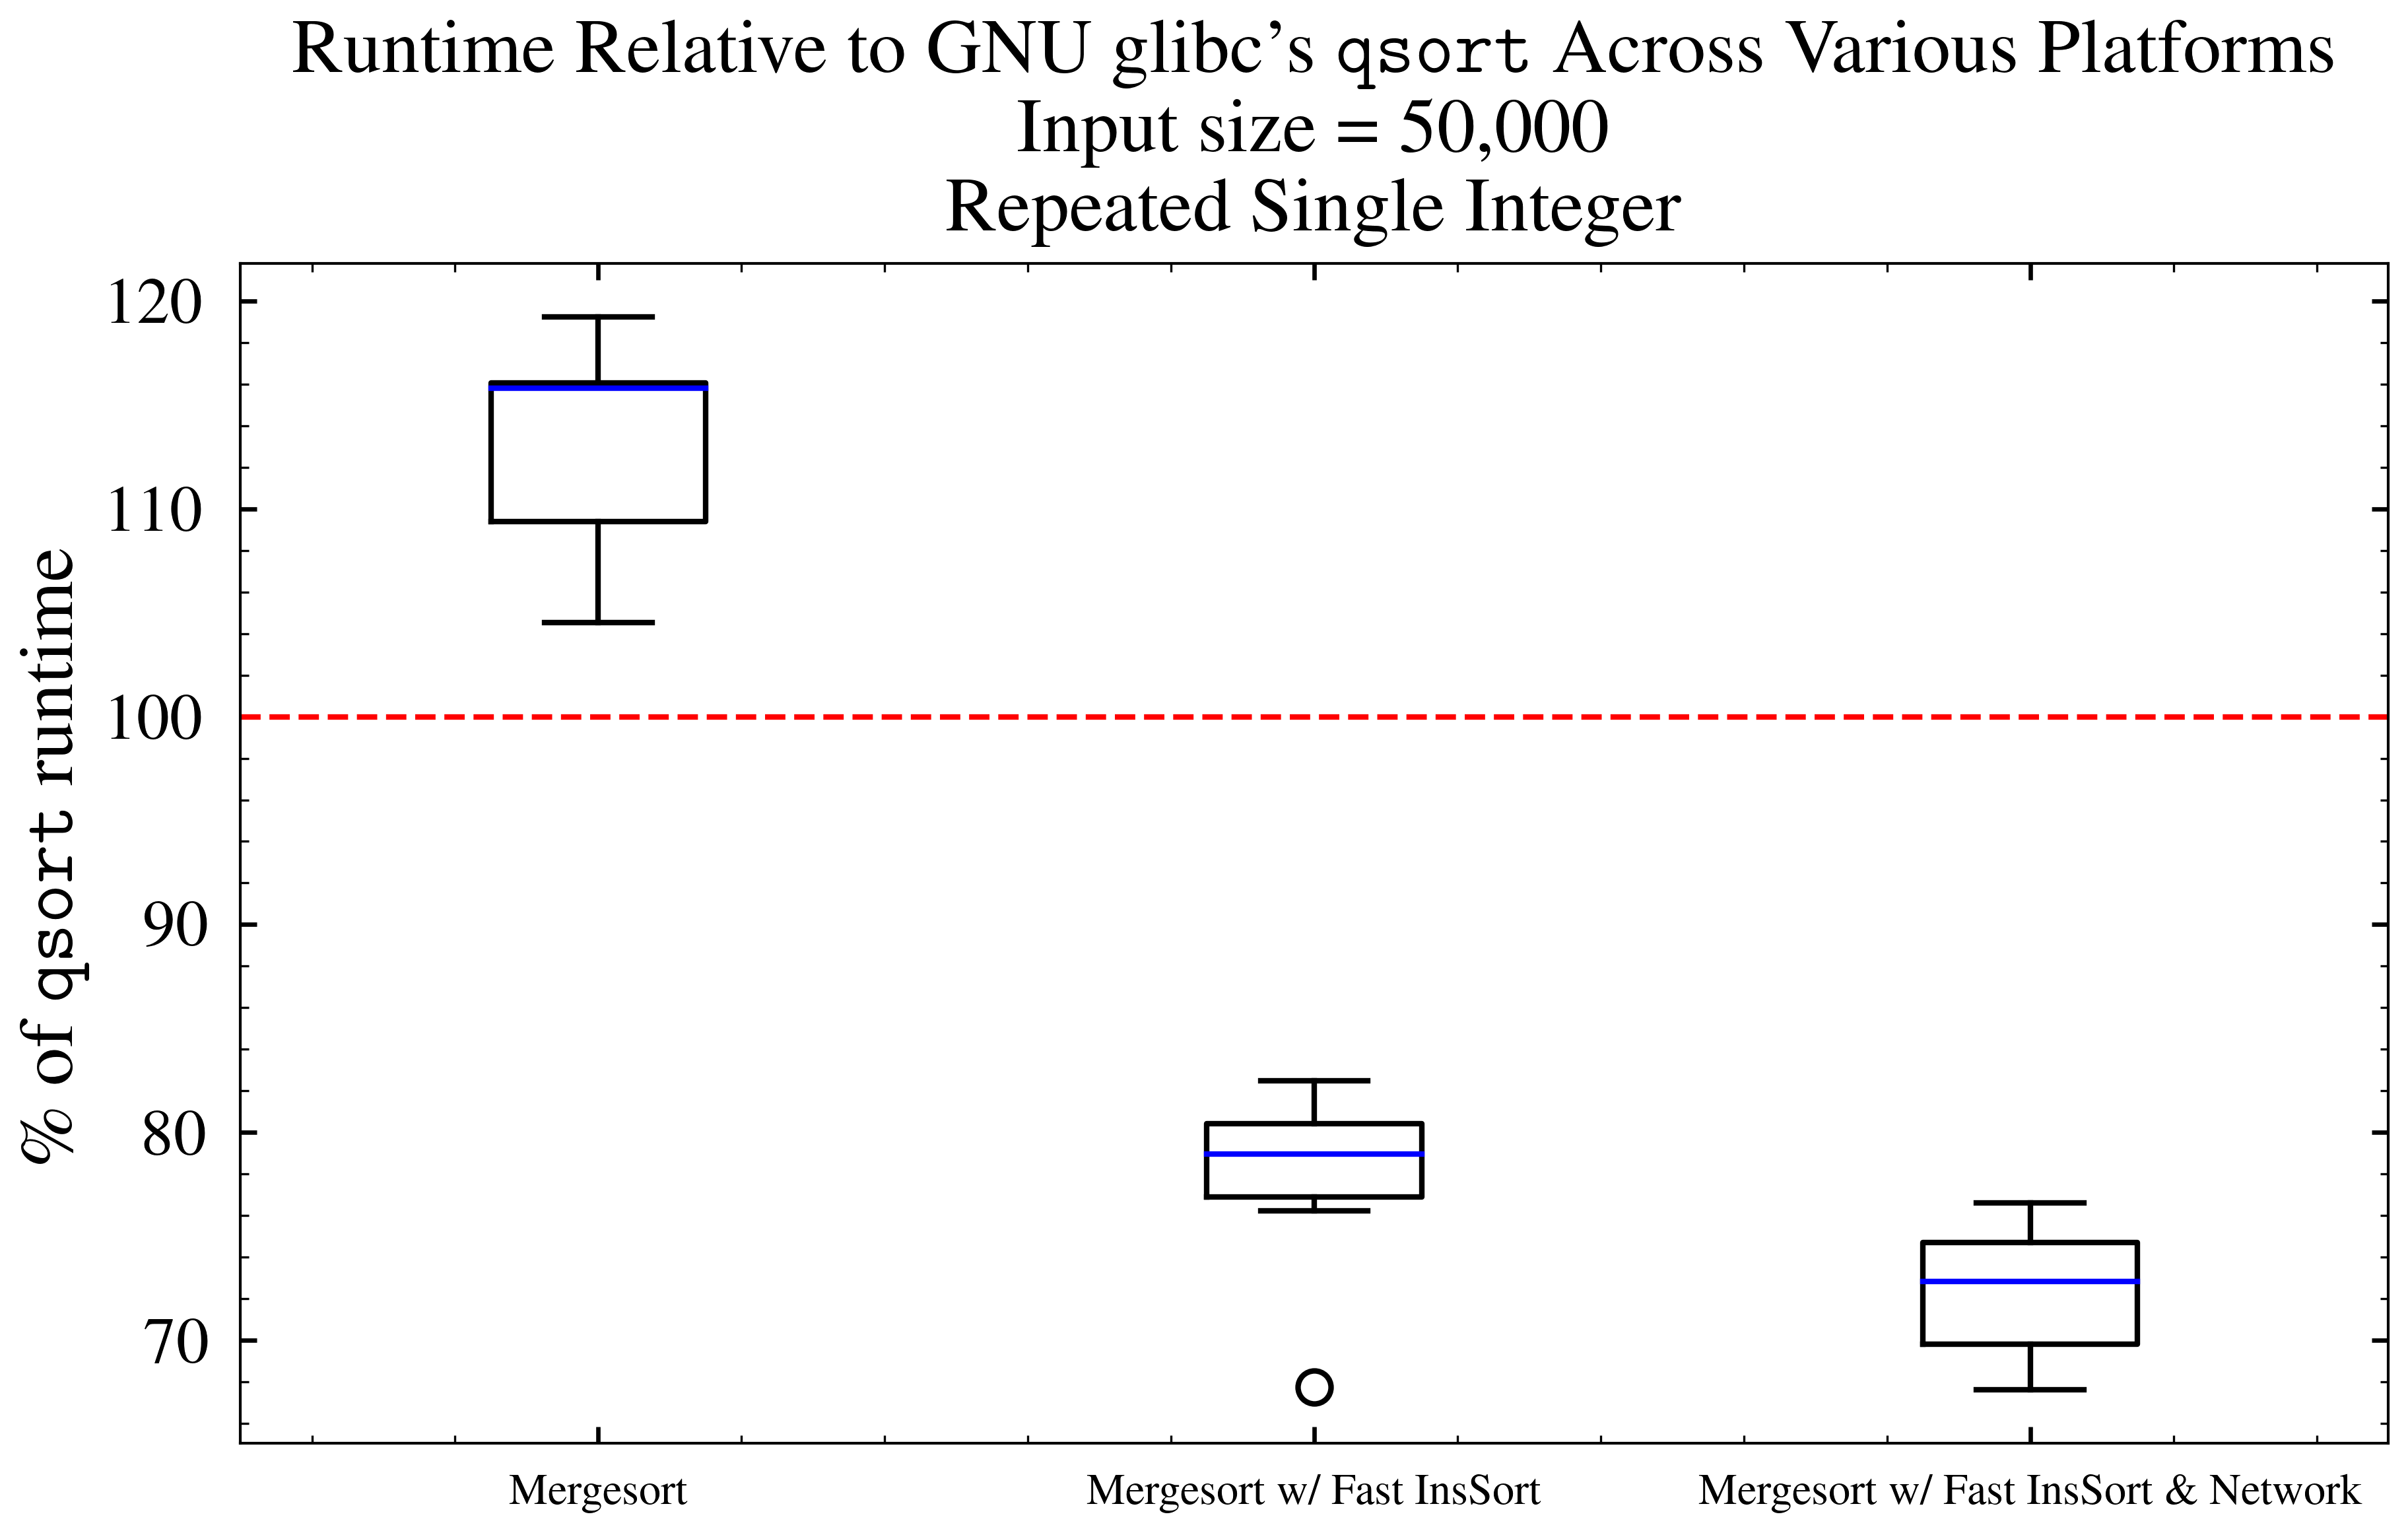
\includegraphics[width=\columnwidth]{../figures/boxplots/1.gen.png}
	\end{multicols}
\end{frame}

\section{Conclusion}
\begin{frame}{Conclusion}
	\begin{itemize}
		\item There is some more performance to be gained.
		\item GNU libc will hopefully adopt these changes.
		\item Repeating testing like this every few years is important, since
		      hardware changes so much.
		\item Trying silly configurations may lead to finding something amazing.
		\item If you really need super high-performance sorting, implement some
		      hand-tailored algorithm instead of relying on glibc.
	\end{itemize}
\end{frame}

\subsection*{Thank You}
\begin{frame}{}
	\centering
	\Huge Questions?

	\vspace{0.3cm}

	\small

	\texttt{https://github.com/uwyo-mallet/Hybrid-Sorting-Optimization}

	\faEnvelope\texttt{jarulsam@uwyo.edu}

	\faGithub\texttt{jarulsamy}

\end{frame}

\end{document}
